\documentclass[a4paper, 12pt]{book}
\usepackage{amsmath}
\usepackage{graphicx}
\usepackage[left=3cm,top=3cm,right=3cm]{geometry}

\renewcommand{\topfraction}{0.85}
\renewcommand{\textfraction}{0.1}
\parindent=0cm

\newcommand{\pr}{\textnormal{P}}




\title{STATS 331 \\
\vspace{3cm}
Introduction to Bayesian Statistics}
\author{Brendon J. Brewer}
\date{}

\begin{document}
\maketitle
\tableofcontents
\section{Prologue}
This course was originally developed by Dr Wayne Stewart (formerly of The
University of
Auckland) and was first offered in 2009 (Figure~\ref{fig:wayne}).
I joined the faculty in July 2012
and took over the course from him. It was good fortune for me that Wayne left
the university as I arrived: if I had been able to choose which undergraduate
course I would most like to teach, it would have been this one!

Wayne is a passionate Bayesian and advocate
for the inclusion of Bayesian statistics in the undergraduate curriculum.
While this edition of the course differs from Wayne's in some ways\footnote{
The differences are mostly cosmetic. 90\% of the content is the same.},
I hope I am able to do the topic justice in an accessible way.

\begin{figure}
\begin{center}
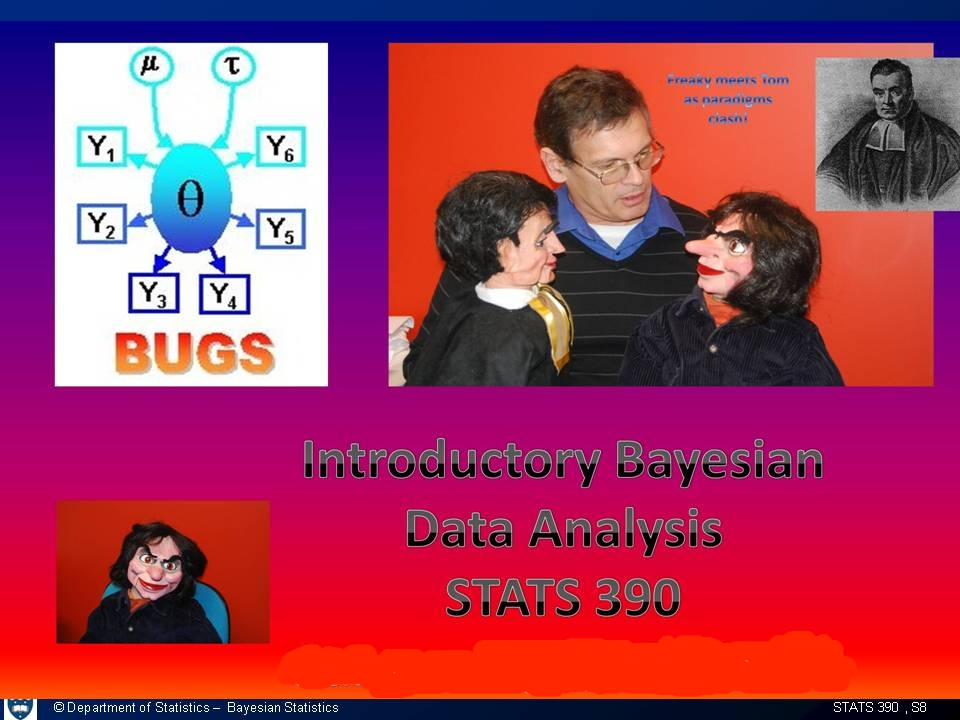
\includegraphics[scale=0.5]{390course.jpg}
\end{center}
\caption{An ad for the original version of this course (then called
STATS 390), showing Wayne Stewart with two ventriloquist dolls, who would
have debates about statistics.\label{fig:wayne}}
\end{figure}

In this course we will use the following software:
\begin{itemize}
\item R ({\tt http://www.r-project.org/}) \\
\item JAGS ({\tt http://mcmc-jags.sourceforge.net/}) \\
\item R-Studio ({\tt http://www.rstudio.org/})
\end{itemize}
You will probably have used R, at least a little bit, in previous statistics
courses. R-Studio is just a nice program used for editing R code, so if you
don't like it, you're welcome to use any other text editor. JAGS is in a
different category: you most likely won't have seen it before.
But don't worry, it's not too difficult to learn and use!

These programs are all free and open source software.
That is, they are free to use, share and modify. They should work on
virtually any operating system including the three most popular:
Microsoft Windows, Mac OS X and GNU/Linux. In previous editions of the course,
WinBUGS was used instead of JAGS. However, WinBUGS has not been updated for
several years, and only works on Microsoft Windows. The differences between
the two are fairly minor, but JAGS has the advantage of being open source and
cross-platform.

\subsection{Bayesian and Classical Statistics}
Throughout this course we will see many examples of Bayesian analysis, and we
will sometimes mention or compare our results with what you get from
{\it classical} or {\it frequentist} statistics, which is the other way of
doing things. You will have seen some classical statistics methods from STATS
10X and 20X, and possibly other courses as well.

Many
people have differing views on the status of these two ways of doing statistics.
In the past, Bayesian statistics was controversial, and you had to be very
brave to use it! Many people were {\bf anti}-Bayesian. Those people are now
rare: instead of Bayesians and anti-Bayesians, it would be more realistic to
say there are now Bayesians and non-Bayesians, and many of the non-Bayesians
would be happy to use Bayesian statistics in some circumstances.
The non-Bayesians would say that
Bayesian statistics is {\it one way} of doing things, and it is a matter of
choice which way you prefer to use. In my opinion, Bayesian
statistics is {\it the right way} to do things, and non-Bayesian methods are
always, at least subtly, wrong, even if they perform well in practice (which
they often do). Sometimes I may give my own opinion on this issue, but
there is one point that you should keep in mind throughout
this course, though, and it is very important:

\begin{center}
\begin{tabular}{|c|}
\hline
{\bf You do not have to agree with me in order to do well in STATS 331!}\\
\hline
\end{tabular}
\end{center}

\subsection{List of Bayesian Statistics Terminology}
Prior probability, posterior probability, prior distribution, posterior
distribution, markov chain monte carlo (MCMC) methods

\subsection{List of Classical/Frequentist Statistics Terminology}
Estimator, Confidence Interval, p-value, bias, bootstrap.


\chapter{Introduction}
Every day, throughout our lives, we are required 
to believe certain things and not to believe other things. This applies not
only to the ``big questions'' of life, but also to trivial matters, and 
everything in between. For example, this morning I boarded the bus to 
university, sure that it would actually take me here and not to Wellington.
How did I know the bus would not take me to Wellington? Well, for starters
I have taken the same bus many times before and it has always taken me to the
university. Another clue was that the bus said ``Midtown'' on it, and a bus
to Wellington would probably have said Wellington, and would not have stopped
at a minor bus stop in suburban Auckland.
None of this evidence {\it proves} that the bus would take me to university,
but it does makes it plausible. Given all these pieces of information, I feel
quite certain that the bus will take me to the city. I feel so certain
about this that the possibility of an
unplanned trip to Wellington never even entered my mind until I decided to
write this paragraph.

Somehow, our brains are very often able to accurately predict the correct answer
to many questions (e.g. the destination of a bus), even though we don't have
all of the available information that we would need to be 100\% certain.
We do this using our experience of the world and our intuition, usually 
without much conscious attention or problem solving. However, there are areas
of study where we can't just use our intuition to make judgments like this.
For example, most of science involves such situations - people tend to be
interested in trying to answer questions that haven't yet been answered!
This is where statistics comes in: to help us in this grey area where we can't
be 100\% certain about things, but we want to do the best we can with our
incomplete information.

\section{Certainty, Uncertainty and Probability}
In the above example, I said things like ``I couldn't be 100\% certain''. The
idea of using a number to describe how certain you are is quite familiar.
For example, contestants on ``Who Wants to be a Millionaire'' often say things
like ``I'm about 80\% sure the answer is A''. There are some interesting
things to notice about this statement. Firstly, it is a subjective statement.
If someone else were in the seat trying to answer the question, they might say
the probability that A is correct is 100\%, because they know the answer!
A third person faced with the same question might say the probability is 25\%,
because they have no idea and only know that one of the four answers
must be correct.

In Bayesian statistics, the interpretation of what {\it probability} means is
that it is a description of {\it how certain you are that some statement is
true}.
If the probability is 1, you are sure that the statement is true. So sure, in
fact, that nothing could ever change your mind (we will demonstrate this later).
If the probability is 0, you
are sure that the statement is false. If the probability is 0.5, then you
are as uncertain as you would be about a fair coin flip. If the probability is
0.95, then you're quite sure the statement is true, but it wouldn't be {\it too}
surprising to you if you found out the statement was false. See
Figure~\ref{fig:probability_scale} for a graphical depiction of probabilities
as degrees of certainty or plausibility.

\begin{figure}
\begin{center}
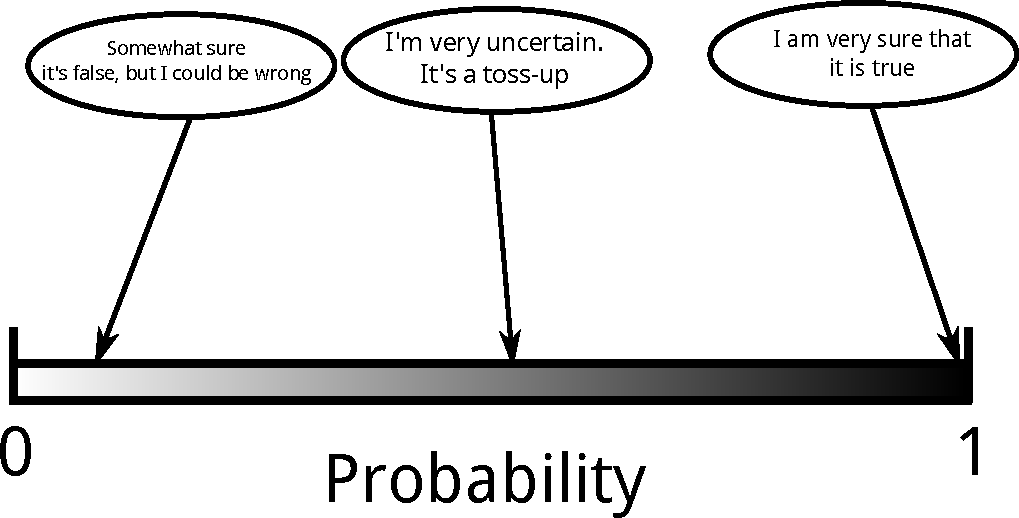
\includegraphics[scale=0.6]{Figures/probability_scale.pdf}
\caption{Probability can be used to describe degrees of certainty, or
how plausible some statement is.\label{fig:probability_scale}}
\end{center}
\end{figure}

\begin{center}
\begin{tabular}{|c|}
\hline
{\bf In Bayesian statistics, probabilities are in the mind, not in the world.}\\
\hline
\end{tabular}
\end{center}

It might sound like there is nothing more to Bayesian statistics than just
thinking about a question and then blurting out a probability that feels
appropriate. Fortunately for us, there's more to it than that! To see why, think
about how you change your mind when new evidence (such as a data set) becomes
available. For example, you may be on ``Who Wants to be a Millionaire?'' and
not know the answer to a question, so you might think the probability that it is
$A$ is 25\%. But if you call your friend using ``phone a friend'', and
your friend says
``it's definitely $A$'', then you would be more confident that it is $A$!

\begin{center}
\begin{tabular}{|c|}
\hline
{\bf When we get new information, we should {\it update} our probabilities.}\\
{\bf Bayesian methods tell us exactly how to do that.}\\
\hline
\end{tabular}
\end{center}

In this course, we will learn how to do {\it data analysis} from a Bayesian
point of view. So while the discussion in this chapter might sound a bit
like philosophy, we will see that using this kind of thinking can give us
new ways of solving practical data analysis problems. The methods we will use
will all have a common structure, so if you are faced with a completely new
data analysis problem one day, you will be able to design your own analysis
methods by using the Bayesian framework. Best of all, the methods make sense
and perform extremely well in practice!





\chapter{First Examples}
We will now look at a simple example that demonstrates all the features of
Bayesian statistics. The problem is quite simple, but we will be able to see
how we start with some probabilities at the beginning of the problem (these are
called {\it prior probabilities}), and how exactly these get updated
into after we get more information (these updated probabilities are called
{\it posterior probabilities}). To help make things more clear, we will
use a table that we will call a {\it Bayes' Box} to help us calculate the
posterior probabilities.

Here is the problem we will use. Suppose that there are two balls in a bag. We know in advance
that at least one of them is black. But we're not sure whether they're both
black, or whether one is black and one is white. These are the two possibilities
we will consider.
To keep things concise, we
can label our two competing hypotheses. We could call them whatever we want,
but I will call them \bb~and \bw. So, at the beginning of the problem, we know
that {\it one and only one} of the following statements/hypothesis is true:\\
\begin{framed}
\bb: Both balls are black\\
\bw: One ball is black and the other is white.
\end{framed}
Suppose an experiment is performed to help us determine
which of these two hypotheses is
true. The experimenter reaches into the bag, pull out one of the balls, and
observes its colour. The result of this experiment is (drumroll please!):
\begin{framed}
$D$: The ball that was removed from the bag was black.
\end{framed}
We will now do a Bayesian analysis of this result.

\section{The Bayes' Box}
A Bayesian analysis starts by choosing some values for the prior probabilities.
We have our two competing hypotheses \bb~and \bw, and we need to choose some
probability values to describe how sure we are that each of these is true.
Since we are talking about two hypotheses, there will be two prior probabilities,
one for \bb~and one for \bw.
For simplicity, we will assume that we don't have much of an idea which is true,
and so we will use the following prior probabilities:
\begin{eqnarray}
P(\bb) &=& 0.5\\
P(\bw) &=& 0.5.
\end{eqnarray}
Pay attention to the notation: the upper case $P$ stands for probability, and if we just
write $P(\texttt{whatever})$, that means we are talking about the
prior probability of {\tt whatever}. We will see the notation for the posterior probability
shortly. Note also that since the two hypotheses are mutually exclusive
(they can't both be true) and exhaustive (one of these is true, it can't be
some undefined third option).
We will almost always consider mutually exclusive and exhaustive hypotheses in
this course\footnote{If this does not appear to be true in a particular problem,
it usually possible to redefine the various hypotheses into a set that {\it are}
mutually exclusive and exhaustive.}.

The choice of 0.5 for the two prior probabilities describes the fact that,
before we did the experiment, we were very uncertain about which of the two
hypotheses was true.
I will now present a {\it Bayes' Box}, which lists all the hypotheses (in this
case
two) that might be true, and the prior probabilities. There are some extra
columns which we haven't discussed yet, which will be needed in order to
figure out the posterior probabilities in the final column.
\begin{table}[h!]
\begin{center}
\begin{tabular}{|c|c|c|c|c|}
\hline
{\bf Hypotheses} & {\tt prior} & {\tt likelihood} &
{\tt prior $\times$ likelihood} & {\tt posterior}\\
\hline
\bb & 0.5 &   &  & \\
\bw & 0.5 &   &  & \\
\hline
Totals: & 1 & & & \\
\hline
\end{tabular}
\end{center}
\end{table}
The first column of a Bayes' Box is just the list of hypotheses we are
considering, in this case there are just two. If you need to construct a Bayes' box for a new problem, just think
about what the possible answers to the problem are, and list them in the first
column. The second column lists the prior probabilities for each of the
hypotheses.
Above, we decided to say that there is a 50\%
probability that \bb~is true and a 50\% probability that \bw~is true, before
we did the experiment, hence the 0.5 values in this column.
The prior column should always sum to 1. Remember, the prior probabilities
only describe our initial uncertainty, before taking into account the
data. Hopefully the data will help by changing these probabilities to
something a bit more decisive!

\subsection{Likelihood}
The third column is called {\it likelihood}, and this is a really important
column where the action happens. The likelihood is a quantity
that will be used for calculating the posterior
probabilities.
In colloquial language, likelihood is synonymous with
probability; it means the same thing. However, in statistics, likelihood is a
very
specific kind of probability. To fill in the third column of the Bayes' Box,
we need to calculate two likelihoods, so you can tell from this that the
likelihood is something that is different for each hypothesis. But what is it
exactly?
\begin{framed}
{\bf The likelihood for a hypothesis is the probability that you would have
observed the data, if that hypothesis were true. The values can be found by
going through each hypothesis in turn, imagining it is true, and asking
``what is the probability of getting the data that I observed?''}
\end{framed}

Here is the Bayes' Box with the likelihood column filled in. I will explain
how these numbers were calculated in a bit more detail in the next subsection.
\begin{table}[h!]
\begin{center}
\begin{tabular}{|c|c|c|c|c|}
\hline
{\bf Hypotheses} & {\tt prior} & {\tt likelihood} &
{\tt h = prior $\times$ likelihood} & {\tt posterior}\\
\hline
{\tt BB} & 0.5 & 1 &  & \\
{\tt BW} & 0.5 & 0.5 &  & \\
\hline
Totals: & 1 & & & \\
\hline
\end{tabular}
\end{center}
\end{table}
If you have taken STATS 210 and used the maximum likelihood method, where you
find the value of a parameter that maximises the likelihood function, that is
the same as the likelihood we use in this course! So you have a head start
in understanding this concept.

\subsection{Finding the Likelihood Values}
We will first calculate the value of the likelihood for the \bb~hypothesis.
Remember, the data we are analysing here is that we chose one of the balls in
the bag ``at random'', and it was black. The likelihood for the \bb~hypothesis is
therefore the probability that we would get a black ball if \bb~is true.

Imagine that \bb~is true. That means both balls are black. What is the probability that
the experiment would result in a black ball? That's easy -- it's 100\%! So we
put the number 1 in the Bayes Box as the likelihood for the \bb~hypothesis.

Now imagine instead that \bw~is true. That would mean one ball is black and the
other is white. If this were the case and we did the experiment, what would be
the probability of getting the black ball in the experiment? Since one of the
two balls is black, the chance of choosing this one is 50\%. Therefore the
likelihood for the \bw~hypothesis is 0.5, so that's why I put 0.5 in the Bayes'
Box for the likelihood for \bw.

In general, the likelihood is the {\it probability of the data that you actually
got, assuming that a particular hypothesis is true}. In this example it was
fairly easy to get the likelihoods directly by asking ``if this hypothesis
were true, what would be the probability of the experiment outcome being the
black ball?''. Sometimes it's not so easy, and it can be helpful to think about
ALL possible experimental outcomes/data you might have seen -- even though
ultimately, you just need to select the one that actually occurred.
Table~\ref{tab:all_data} shows an example of this process.

\begin{table}[h!]
\begin{center}
\begin{tabular}{|c|c|c|}
\hline
{\bf Hypotheses} & {\bf Possible Data} & {\bf Probability} \\
\hline
{\tt BB} & {\color{blue} Black Ball} & {\color{blue} 1}\\
         & White Ball & 0 \\
\hline
{\tt BW} & {\color{blue} Black Ball} & {\color{blue} 0.5} \\
         & White Ball & 0.5 \\
\hline
\end{tabular}
\caption{This table demonstrates a method for calculating the likelihood
values, by considering not just the data that actually occurred, but all
data that might have occurred. Ultimately, it is only the probability of the
data that actually occurred that matters, so this is highlighted in blue.
\label{tab:all_data}}
\end{center}
\end{table}
The fact that only the blue probabilities in Table~\ref{tab:all_data} enter the
Bayes' Box calculation is related to the {\it likelihood principle} which is
discussed in lectures. Note also that in Table~\ref{tab:all_data}, the
probabilities for the different possible data sets add to 1 within each
hypothesis, but the sum of the blue ``selected'' likelihood values is not 1
(it is meaningless, in fact).

\subsection{The Mechanical Part}
The third column of the Bayes' Box is the product of the prior probabilities
and the likelihoods, calculated by simple multiplication. The result will be
called ``prior times likelihood'', but occasionally we will use the letter $h$
for these quantities. This is the {\it unnormalised} posterior: it does not sum
to 1 as the posterior probabilities should, but it is at least proportional to
the actual posterior probabilities.

To find the posterior probabilities, we take the {\tt prior $\times$ likelihood}
column and divide it by its sum, producing numbers that do sum to 1: the final
posterior probabilities, which were the goal all along. The completed Bayes'
Box is shown below:

\begin{table}[h!]
\begin{center}
\begin{tabular}{|c|c|c|c|c|}
\hline
{\bf Hypotheses} & {\tt prior} & {\tt likelihood} &
{\tt h = prior $\times$ likelihood} & {\tt posterior}\\
\hline
{\tt BB} & 0.5 & 1 & 0.5 & 0.667\\
{\tt BW} & 0.5 & 0.5 & 0.25  & 0.333\\
\hline
Totals: & 1 & & 0.75 & 1\\
\hline
\end{tabular}
\end{center}
\end{table}

\subsection{Interpretation}
The posterior probabilities of the hypotheses are proportional to the prior probabilies
and the likelihoods. A high prior probability will help a hypothesis have a high
posterior probability. A high likelihood value also helps.
To understand what this means about reasoning, consider
the meanings of the prior and the likelihood. There are two things that can
contribute to a hypothesis being plausible:
\begin{itemize}
\item If the prior probability is high, that is, the hypotheses was {\it already}
plausible, before we got the data.
\item If the hypotheses {\it predicted the data} well. That is, the data that
occurs was what we would have expected to observe if the hypothesis is true.
\end{itemize}
I hope you agree that this is all very sensible.

\section{Bayes' Rule}
Bayes' rule is an equation from probability theory, shown in
Figure~\ref{fig:bayes_neon}. The various terms in Bayes' rule are all
probabilities, but notice that there are conditional probabilities in there.
For example, the left hand side of the equation is $P(A|B)$ and that means
the probability of $A$ {\bf given} $B$; that is, it's the probability of $A$
after taking into account the information $B$. In other words,
$P(A|B)$ is a posterior probability, and Bayes' rule tells us how to calculate
it from other probabilities.
\begin{figure}[h]
\begin{center}
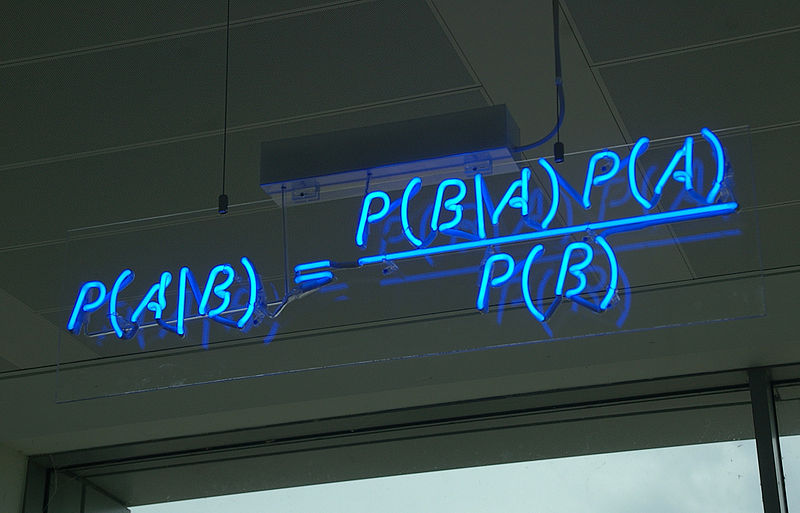
\includegraphics[scale=0.4]{Figures/bayes_neon.jpg}
\caption{A blue neon sign displaying Bayes' rule.
You can use it to calculate the probability of $A$ {\it given} $B$,
if you know the values of some other probabilities on the right hand side.
Image credit: Matt Buck. Obtained from Wikimedia Commons.
\label{fig:bayes_neon}}
\end{center}
\end{figure}
Bayes' rule is true for {\it any} statements $A$ and $B$. If you took the
equation in Figure~\ref{fig:bayes_neon} and replaced $A$ with
``K\={a}k\={a}p\={o} will survive beyond 2050'' and $B$ with
``I had coffee this morning'', the
resulting equation would still be true\footnote{Albeit not very interesting,
because
whether or not I had coffee doesn't tell you much about the survival prospects
of endangered New Zealand parrots.}.

It is helpful to relabel $A$ and $B$ in Bayes' rule to give a more clear
interpretation of how the equation is to be used. In this version of Bayes'
rule (which is one you should commit to memory), $A$ has been replaced by $H$,
and $B$ has been replaced by $D$. The reason for these letters is that you should
interpret $H$ as {\it hypothesis} and $D$ as {\it data}. Then you can interpret
Bayes' rule as telling you the probability of a hypothesis given some data --
that is, a posterior probability.
\begin{eqnarray}
P(H|D) = \frac{P(H)P(D|H)}{P(D)}
\end{eqnarray}
In Bayesian statistics, most of the terms in Bayes' rule have special names.
Some of them even have more than one name, with different scientific
communities preferring different terminology. Here is a list of the
various terms and the names we will use for them:
\begin{itemize}
\item $P(H|D)$ is the {\bf posterior probability}. It describes how certain
or confident we are that
hypothesis $H$ is true, given that we have observed data $D$. Calculating
posterior probabilities is the main goal of Bayesian statistics!
\item $P(H)$ is the {\bf prior probability}, which describes how sure we were
that $H$ was true, before we observed the data $D$.
\item $P(D|H)$ is the {\bf likelihood}. If you were to assume that $H$ is true,
this is the probability that you would have observed data $D$.
\item $P(D)$ is the {\bf marginal likelihood}. This is the probability that you
would have observed data $D$, {\it whether $H$ is true or not}.
\end{itemize}
Since you may encounter Bayesian methods outside of STATS 331, I have included
an Appendix called ``Rosetta Stone'' that lists some common alternative
terminology.

In the above example, we did some calculations to work out the numbers in the
Bayes' Box, particularly the posterior probabilities, which are the ultimate
goal of the calculation. {\it What we were actually doing in these calculations
was applying Bayes' rule}. We actually applied Bayes' rule twice, once to
compute $P(\bb | D)$ and a second time to calculate $P(\bw | D)$.

\begin{framed}
{\bf When you use a Bayes' Box to calculate posterior probabilities,
you are really just applying Bayes' rule a lot of times:
once for each hypothesis listed in the first column.}
\end{framed}

\section{Phone Example}
\subsection{The Question}
This example is based on Question 1 from the 2012 final exam of STATS 331. The
idea for this question was based on an example in David MacKay's wonderful book
``Information Theory, Inference and Learning Algorithms''
(available online as a free PDF download -- you're welcome to check it out, but
it is a large book and only about 20\% of it is related to this course!).

You move into a new house which has a phone
installed. You can't remember the phone number, but you suspect it
might be {\tt 555-3226} (some of you may recognise
this as being the phone number for Homer Simpson's ``Mr Plow'' business).
To test this hypothesis, you carry out an experiment
by picking up the phone and dialing {\tt 555-3226}.

If you are correct about
the phone number, you will definitely hear a busy signal because you are calling
yourself.
If you are incorrect, the probability of hearing a busy signal is $1/100$.
However, all of that is only true if you assume the phone is working -- and it
might be broken! If the phone is broken, it will always give a busy signal.

When you do the experiment, you do actually get the busy signal.
Find the posterior probability the following four hypotheses:
\begin{table}[h!]
\begin{center}
\begin{tabular}{|c|c|c|c|}
\hline
Hypothesis & Description & Prior Probability\\
\hline
$H_1$ & Phone is working and {\tt 555-3226} is correct & 0.4\\
$H_2$ & Phone is working and {\tt 555-3226} is incorrect & 0.4\\
$H_3$ & Phone is broken and {\tt 555-3226} is correct & 0.1\\
$H_4$ & Phone is broken and {\tt 555-3226} is incorrect & 0.1\\
\hline
\end{tabular}
\caption{The four hypotheses about the state of the phone and the phone
number. The prior probabilities are also given.\label{tab:phone}}
\end{center}
\end{table}

\subsection{Solution}
We will go through the solution using a Bayes' Box. The four hypotheses listed
in Table~\ref{tab:phone} are mutually exclusive and exhaustive, so we can fill
out the first two columns of a Bayes' Box right away:
\begin{table}[h!]
\begin{center}
\begin{tabular}{|c|c|c|c|c|}
\hline
{\bf Hypotheses} & {\tt prior} & {\tt likelihood} &
{\tt prior $\times$ likelihood} & {\tt posterior}\\
\hline
$H_1$ & 0.4 &  &  & \\
$H_2$ & 0.4 &  &  & \\
$H_3$ & 0.1 &  &  & \\
$H_4$ & 0.1 &  &  & \\
\hline
Totals: & 1 & & & \\
\hline
\end{tabular}
\end{center}
\end{table}
The next thing we need are the likelihoods. The data was that we got the busy
signal, so we need to work out $P(\textnormal{busy signal} | H)$ for each $H$
in the problem (there are four of them). Let's start (naturally!) with $H_1$.

If we assume $H_1$ is true, then the phone is working and {\tt 555-3226} is the
correct phone number. In that case, we would definitely get a busy signal. So
$P(\textnormal{busy signal} | H_1) = 1$ is our first likelihood value.
Next, let's imagine that $H_2$ is true, so the phone is working, but
{\tt 555-3226} is not the right phone number. In this case, it is given in the
question that the probability of getting a busy signal is $1/100$ or 0.01.
Therefore $P(\textnormal{busy signal} | H_2) = 0.01$, and that's our second
likelihood. The likelihoods for $H_3$ and $H_4$ are quite straightforward
because they both imply the phone is broken, and that a busy signal is certain.
Therefore $P(\textnormal{busy signal} | H_3) = P(\textnormal{busy signal} | H_4) = 1$.
We have our four likelihoods, and can proceed to work out everything in the
Bayes' Box, including the main goal -- the posterior probabilities! Here it is:
\begin{table}[h!]
\begin{center}
\begin{tabular}{|c|c|c|c|c|}
\hline
{\bf Hypotheses} & {\tt prior} & {\tt likelihood} &
{\tt prior $\times$ likelihood} & {\tt posterior}\\
\hline
$H_1$ & 0.4 & 1 &  0.4 & 0.662\\
$H_2$ & 0.4 & 0.01 & 0.004 & 0.00662\\
$H_3$ & 0.1 & 1 & 0.1 & 0.166\\
$H_4$ & 0.1 & 1 & 0.1 & 0.166\\
\hline
Totals: & 1 & & 0.604 & 1\\
\hline
\end{tabular}
\end{center}
\end{table}

To conclude this phone problem, I should admit that
I actually calculated the numbers in the Bayes' Box using R. My code is shown
below. Obviously in the
2012 exam the students had to use their calculators.
\begin{framed}
\begin{verbatim}
> prior = c(0.4, 0.4, 0.1, 0.1) # Vector of prior probs
> lik = c(1, 0.01, 1, 1)        # Vector of likelihoods
> h = prior*lik
> Z = sum(h)                    # Sum of prior times likelihood
> post = prior*lik/Z            # Normalise to get posterior
> # Look at all the results
> print(prior)
[1] 0.4 0.4 0.1 0.1
> print(lik)
[1] 1.00 0.01 1.00 1.00
> print(h)
[1] 0.400 0.004 0.100 0.100
> print(Z)
[1] 0.604
> print(post)
[1] 0.662251656 0.006622517 0.165562914 0.165562914
\end{verbatim}
\end{framed}
Now let's try to see if this makes sense. There are many things we could think
about, but let's just consider the question of whether
the phone is working or not. The first two hypotheses correspond to the phone
being in a working state. The prior probability that the phone is working is
therefore:
\begin{eqnarray}
P(\textnormal{phone working}) &=& P(H_1 \textbf{ or } H_2)\\
&=& P(H_1) + P(H_2)\\
&=& 0.4 + 0.4\\
&=& 0.8.
\end{eqnarray}
The posterior probability is worked out in a similar way, but using the posterior
probabilities instead of the prior ones:
\begin{eqnarray}
P(\textnormal{phone working}|\textnormal{busy signal}) &=& P(H_1 \textbf{ or } H_2 | \textnormal{busy signal})\\
&=& P(H_1|\textnormal{busy signal}) + P(H_2|\textnormal{busy signal})\\
&=& 0.662 + 0.00662\\
&=& 0.6689.
\end{eqnarray}
Our probability that the phone is working has gone down a little bit as a result of this
evidence! That makes sense to me -- a busy signal is what you would expect to
happen if the phone was broken. This data doesn't {\it prove} the phone is
broken, but it does point in that direction a little bit.

\section{Important Equations to Remember}
Bayes' rule for a single hypothesis $H$ given data $D$:
\begin{eqnarray}
P(H|D) = \frac{P(H)P(D|H)}{P(D)}
\end{eqnarray}
This gives the posterior probability $P(H|D)$ in terms of the prior probability
$P(H)$, the likelihood $P(D|H)$ and the ``marginal likelihood'' $P(D)$ in the
denominator. To obtain $P(H)$, think about your prior beliefs (which may
indicate a large amount of uncertainty, or may be already well informed based
on previous data sets). To obtain $P(D|H)$, think about what the experiment is
doing: If $H$ is true, what data would you expect to see and with what
probabilities?

The denominator is the probability of obtaining the data $D$ but without
assuming that $H$ is either true or false. This is obtained using the sum rule.
There are two ways that the data $D$ could occur: either via the route of $H$
being true (this has probability $P(H)P(D|H)$) or via the route of $H$ being
false (this has probability $P(\bar{H})P(D|\bar{H})$). These two ways are
mutually exclusive, so we can add their probabilities:
\begin{eqnarray}
P(D) = P(H)P(D|H) + P(\bar{H})P(D|\bar{H}).
\end{eqnarray}

The Bayes' rule from above can be applied to a whole set
of hypotheses (that are mutually exclusive and exhaustive). If we applied the
above equation to $N$ hypotheses
$H_1, H_2, ..., H_N$, given data $D$, we would get the following for the posterior
probability of each hypothesis $H_i$ (for $i=1, 2, ..., N$):
\begin{eqnarray}
P(H_i|D) &=& \frac{P(H_i)P(D|H_i)}{P(D)}
\end{eqnarray}
The denominator $P(D)$ can again be obtained using the sum rule. There are $N$
mutually exclusive ways that the data $D$ could have occurred: via $H_1$ being
true, or via $H_2$ being true, etc. Adding the probabilities of these gives:
\begin{eqnarray}
P(D) &=& \sum_{i=1}^N P(H_i)P(D|H_i).
\end{eqnarray}
If you find all the mathematics a bit much right now, just remember that
Following the steps for making a Bayes' Box is equivalent to applying
Bayes' rule in this form!. The $P(H_i)$ values are the prior probability column, the
$P(D|H_i)$ values are the likelihood column, and the denominator is the
sum of the prior times likelihood column. The probabilities that go in a Bayes'
Box (in general) are given in Table~\ref{tab:general_bayes_box}.

\begin{table}[ht!]
\begin{center}
\begin{tabular}{|c|c|c|c|c|}
\hline
{\bf Hypotheses} & {\tt prior} & {\tt likelihood} &
{\tt prior $\times$ likelihood} & {\tt posterior}\\
\hline
$H_1$ & $P(H_1)$ & $P(D|H_1)$ & $P(H_1)\times P(D|H_1)$ & $P(H_1|D)$\\
$H_2$ & $P(H_2)$ & $P(D|H_2)$ & $P(H_2)\times P(D|H_2)$ & $P(H_2|D)$\\
\ldots & \ldots & \ldots & \ldots & \ldots\\
\hline
Totals: & 1 & & $P(D)$ & 1\\
\hline
\end{tabular}
\caption{A general Bayes' Box. Using Bayes' rule or making a Bayes' Box are
actually the same thing, and this table can be used to identify the
terms.\label{tab:general_bayes_box}}
\end{center}
\end{table}


\chapter{Parameter Estimation}
One of the most important ways of using Bayes' rule is in the topic
called {\it parameter estimation}. Parameter estimation is a fairly common
situation in statistics. In fact, it is possible to interpret almost any
problem in statistics as a parameter estimation problem and approach it
in this way!

Firstly, what is a parameter? Well, it is just a fancy term for a quantity or
a number that is unknown. For example, how many people are currently in New
Zealand? Well, a Google search suggests 4.405 million. But that does not mean
there are {\bf exactly} 4,405,000 people. It could be a bit more or a bit
less. Maybe it is 4,405,323, or maybe it is 4,403,886. We don't really know.
We could call the true number of people in New Zealand right now $\theta$, or
we could use some other letter or symbol if we liked.

The key is to realise that we can use the Bayes Box like in previous chapters,
but now, our list of possible hypotheses is a list of possible values for
the unknown parameter. For example, a Bayes Box for the precise number of
people in New Zealand might look something like this:
\begin{table}[h!]
\begin{center}
\begin{tabular}{|c|c|c|c|c|}
\hline
{\bf Possible Hypotheses} & {\tt prior} & {\tt likelihood} &
{\tt prior $\times$ likelihood} & {\tt posterior}\\
\hline
\ldots & \ldots & \ldots & \ldots & \ldots\\
$\theta = 4404999$ & 0.000001 & \ldots   & \ldots  & \ldots\\
$\theta = 4405000$ & 0.000001 & \ldots   & \ldots  & \ldots\\
$\theta = 4405001$ & 0.000001 & \ldots   & \ldots  & \ldots\\
$\theta = 4405002$ & 0.000001 & \ldots   & \ldots  & \ldots\\
$\theta = 4405003$ & 0.000001 & \ldots   & \ldots  & \ldots\\
$\theta = 4405004$ & 0.000001 & \ldots   & \ldots  & \ldots\\
$\theta = 4405005$ & 0.000001 & \ldots   & \ldots  & \ldots\\
$\theta = 4405006$ & 0.000001 & \ldots   & \ldots  & \ldots\\
\ldots & \ldots & \ldots & \ldots & \ldots\\
\hline
Totals: & 1 & & \ldots & 1\\
\hline
\end{tabular}
\end{center}
\end{table}
There are a few things to note about this Bayes' box. Firstly, that it is big.
There are lots of possible hypotheses, corresponding to possible values for
$\theta$. The prior probabilities I have put in the 2nd column were for
illustration purposes. 

\section{Parameter Estimation: Bus Example}
This is a beginning example of parameter estimation from a Bayesian point of
view. It shows the various features that are always present in a Bayesian
analysis: prior probabilities, likelihood, and posterior probabilities.

After moving to Auckland, I decided that I would take the bus to work
each day. However, I wasn't very confident with the bus system, so for the first
week I just took the first bus that came along and was heading in the right
direction (towards the city).

{\bf Here's the question}. In the first week, I caught 5 morning buses.
Of these 5 buses, two of them took me to the right place, while three of them
took me far from work, leaving me with an extra 20 minute walk. Given this
information, 




Discrete
Bayes Box

Bus example

\begin{table}
\begin{center}
\begin{tabular}{|c|c|c|c|c|}
\hline
\tt{Possible Values} & \tt{Prior} & \tt{Likelihood} & \tt{h} & \tt{Posterior}\\
$\theta$ & $P(\theta)$ & $P(x|\theta)$ & $P(\theta)P(x|\theta)$ & $P(\theta|x)$\\
\hline
0 & 0.0909 & & &\\
0.1 & 0.0909 & & &\\
0.2 & 0.0909 & & &\\
0.3 & 0.0909 & & &\\
0.4 & 0.0909 & & &\\
0.5 & 0.0909 & & &\\
0.6 & 0.0909 & & &\\
0.7 & 0.0909 & & &\\
0.8 & 0.0909 & & &\\
0.9 & 0.0909 & & &\\
1 & 0.0909 & & &\\
\hline
Totals & 1 & & & 1\\
\hline
\end{tabular}
\end{center}
\end{table}

Continuous?


\chapter{Parameter Estimation: Analytical Methods}
Analytical methods are those that can be carried out with a pen and paper,
the ``old school'' way before we all started using computers. There are some
problems in Bayesian statistics that can be solved in this way, and we will
see one or two of them in this course.

Let's look at the {\it binomial likelihood} problem again, with the familiar
bus example. Out of $N=5$ attempts at a ``repeatable'' experiment, there were
$x=2$ successes. From this, we want to infer the value of $\theta$, the
success probability that applied on each trial. Because of its meaning, we know
with 100\% certainty that $\theta$ must be between 0 and 1 (inclusive).

Recall that, if we knew the
value of $\theta$ and wanted to predict the data $x$ (regarding $N$ as being
known in advance), then we would use the binomial distribution:
\begin{eqnarray}
p(x|\theta) &=& \left(\begin{array}{c}N \\ x\end{array}\right)
\theta^x\left(1-\theta\right)^{N - x}.\label{eq:binomial_likelihood}
\end{eqnarray}
This is the probability mass function for $x$. Since there are five trials
($N=5$), the number of successes $x$ must be one of 0, 1, 2, 3, 4, or 5.
If $\theta$ is a high number close to one, then we would expect the resulting
value of the data $x$ to be something high like 4 or 5. Low values for $x$ would
still be possible but they would have a small probability. If $\theta$ is a
small number, we would expect the data to be 0, 1, or 2, with less probability
for more successes than that. This is just saying in words what is written
precisely in Equation~\ref{eq:binomial_likelihood}. The probability distribution
for the data $x$ is plotted in Figure~\ref{fig:binomial} for three illustrative
values of the parameter $\theta$.
\begin{figure}[h!]
\begin{center}
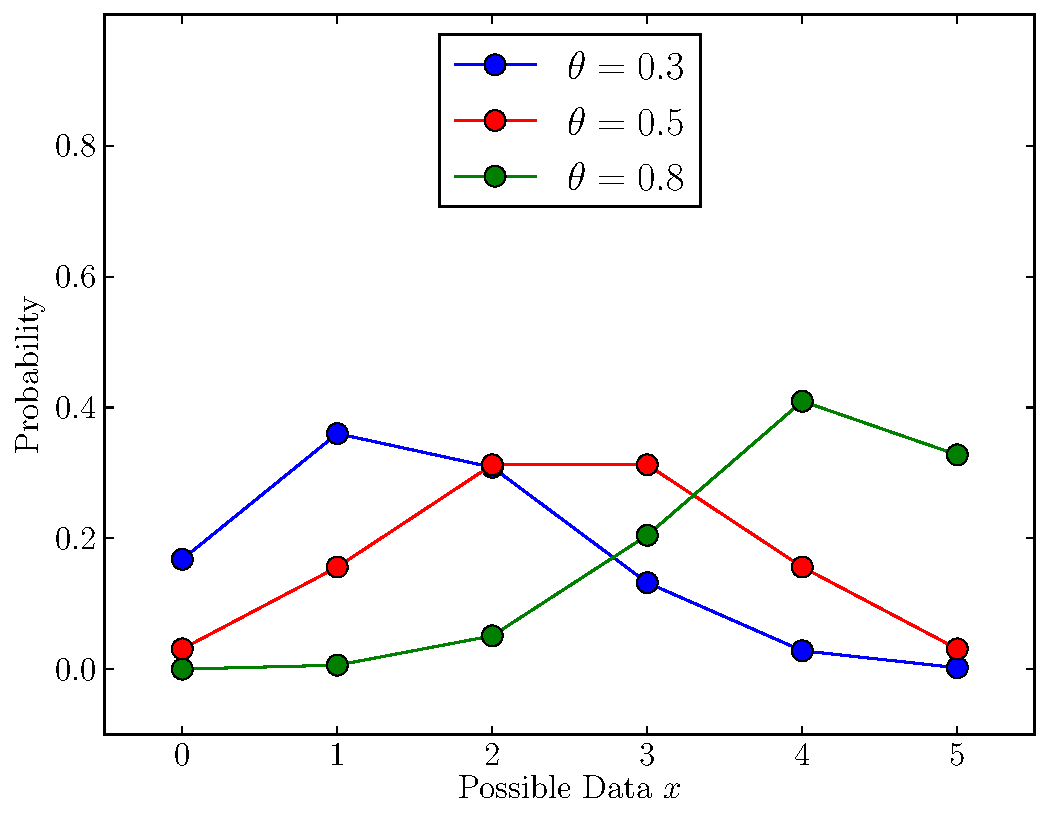
\includegraphics[scale=0.6]{Figures/binomial.pdf}
\caption{\label{fig:binomial}}
\end{center}
\end{figure}

Let's use a uniform prior for $\theta$.
The equation for a uniform probability density is:
\begin{eqnarray}
p(\theta) &=& \left\{
\begin{array}{lr}
1, & 0 \leq \theta \leq 1\\
0, & \textnormal{otherwise}
\end{array}
\right.\label{eq:uniform}
\end{eqnarray}
To find the posterior probability density for $\theta$, we use the ``parameter
estimation'' form of Bayes' rule:
\begin{eqnarray}
\textnormal{posterior} \propto \textnormal{prior} \times \textnormal{likelihood}\\
p(\theta|x) \propto p(\theta)p(x|\theta).
\end{eqnarray}
We already wrote down the equations for the prior and the likelihood, so we
just need to multiply them together.
\begin{eqnarray}
p(\theta|x) &\propto& p(\theta)p(x|\theta)\\
&\propto& 1 \times \left(\begin{array}{c}N \\ x\end{array}\right)
\theta^x\left(1-\theta\right)^{N - x}
\end{eqnarray}
as long as $\theta \in [0, 1]$. There is a handy tip you can use a lot of the
time when working things out analytically. Notice that the ``parameter estimation''
form of Bayes' rule has a proportional sign in it, not an equals sign. That's
because the prior times the likelihood can't actually be the posterior
distribution because it may not be normalised -- the sum or integral is not 1.
However, the equation still gives the correct shape of the probability density
function: the way it depends on $\theta$. The reason this is helpful is that
you can save ink: if there are some factors out the front of your expression
that don't involve the parameter (in this case, $\theta$), you can ignore them!
The proportional sign will take care of them. In this case, it means we can
forget about the pesky ``$N$ choose $x$'' term, and just write:
\begin{eqnarray}
p(\theta|x) &\propto& \theta^x\left(1-\theta\right)^{N - x}\\
&\propto& \theta^2\left(1-\theta\right)^3.
\end{eqnarray}
The final step was to substitute in the actual values of $N$ and $x$ instead of
leaving the symbols there. That's it! We have the correct shape of the
posterior distribution.

\section{Statistician's Notation}
While it is very helpful to know the full equations for different kinds of
probability distributions (both discrete ones and continuous ones), if you only
want to say what a distribution is. Instead of saying ``the prior for $\theta$
is uniform between 0 and 1'', or giving the formula for the prior distribution
(Equation~\ref{eq:uniform}), you can write:
\begin{eqnarray}
\theta \sim \textnormal{Uniform}(0, 1)
\end{eqnarray}
or, even more concisely:
\begin{eqnarray}
\theta \sim U(0, 1).
\end{eqnarray}
This notation conserves ink, and is good for quick communication. It is also
very helpful because when we come to use JAGS in later chapters, it likes
things to be written this way.

We can also write the binomial likelihood in this way, instead of writing out
the full equation. We can write:
\begin{eqnarray}
x | \theta \sim \textnormal{Binomial}(N, \theta)
\end{eqnarray}
This says that, if we knew the value of $\theta$, $x$ would have a binomial
distribution with $N$ trials and success probability $\theta$. We can also
make this more concise:
\begin{eqnarray}
x \sim \textnormal{Bin}(N, \theta)
\end{eqnarray}
The differences here are that ``Binomial'' has been shortened to ``Bin'' and
the ``given $\theta$'' part has been left out. However, we see that there is
a $\theta$ is present on the right hand side, so the ``given $\theta$'' must
be understood implicitly.


\chapter{Summarising the Posterior Distribution}
The posterior distribution is the full answer to any Bayesian problem. It gives
a complete description of our state of knowledge and our uncertainty about the
value(s) of unknown
parameters. From the posterior distribution, we can calculate any probability
we want. For example, if we had a posterior distribution $p(\theta|x)$ and we
wanted to know the probability that $\theta$ is greater than or equal to 100, we could do:
\begin{eqnarray}
P(\theta \geq 100 | x) &=& \int_{100}^\infty p(\theta | x) \, dx
\end{eqnarray}
or
\begin{eqnarray}
P(\theta \geq 100 | x) &=& \sum_{100}^\infty p(\theta | x)
\end{eqnarray}
depending on whether the set of possible $\theta$ values is continuous or
discrete. We could also work out the probability of anything else.
However, the posterior distribution is sometimes too much
information for us to think about easily. Maybe a giant list of $\theta$
values and probabilities isn't easy to digest. Sometimes,
we need to {\it summarise} the posterior distribution to help us
communicate our results with others. A giant Bayes' Box (or a million MCMC
samples of the parameter, we'll see that later), might technically
contain everything we want, but it's not easy to talk about.

For example, say you were trying to estimate
a parameter, and a colleague asked you to state your uncertainty about the
parameter. Well, your posterior distribution might be complicated. It might
have bumps and wiggles in it, or some other kind of structure. If there were
two or more unknown parameters, there might be dependence in the posterior
distribution. In some cases there might even me multiple separate peaks!
Figure~\ref{fig:complicated_posterior} shows an example of what a complicated
posterior distribution might look like. If this was your result, your colleague
might not care about all the little wiggles in this plot. They just want to know
the ``big picture'' of your results.
\begin{figure}[h!]
\begin{center}
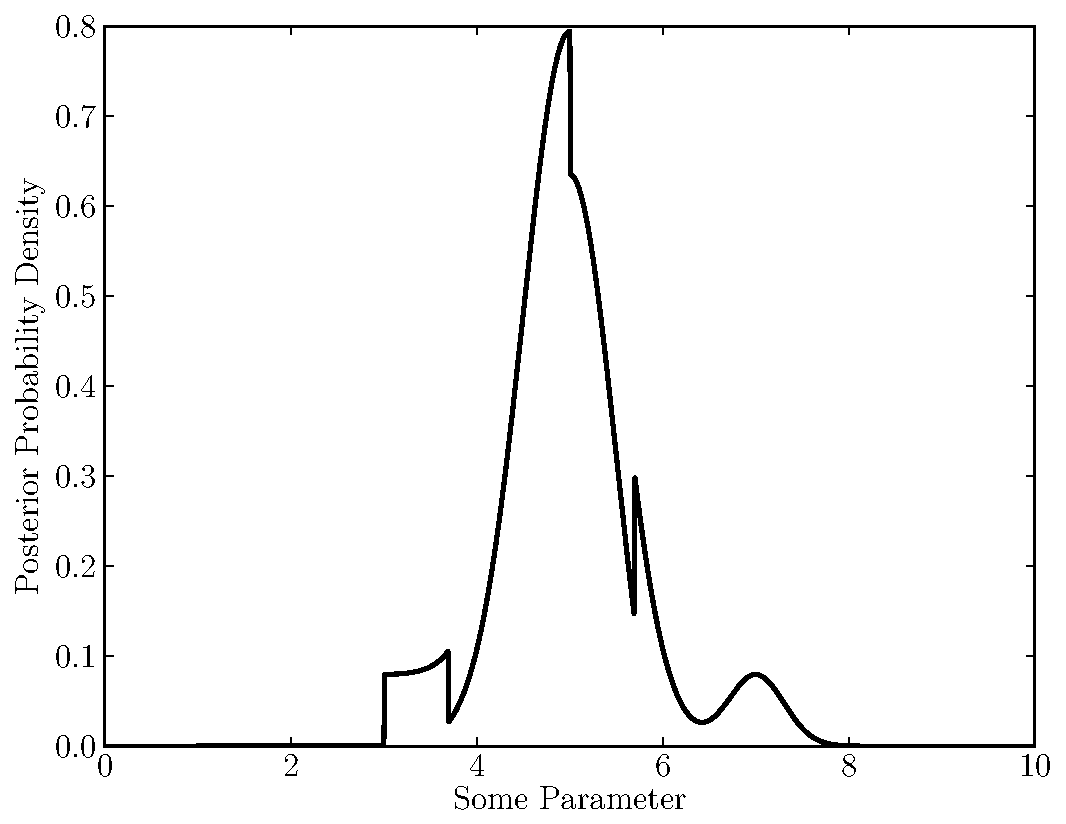
\includegraphics[scale=0.6]{Figures/complicated_posterior.pdf}
\caption{\it A complicated posterior distribution. When communicating with others,
it is often useful to summarise the posterior distribution with a few numbers. In
this case, something like ``the parameter = $5 \pm 1$'' might be a useful summary.
\label{fig:complicated_posterior}}
\end{center}
\end{figure}

The idea of summarising the posterior distribution is very closely related to
the idea of summarising a data set, which you probably encountered when you
studied descriptive statistics.
\begin{framed}
{\bf In descriptive statistics, you often make summaries of a complex data set
(e.g. the mean and the standard deviation) so that you can communicate about
the data set in a concise way. In Bayesian statistics, you often do a similar
thing, but instead of giving a concise description of the {\it data}, you give a
concise description of the {\it posterior distribution}.}
\end{framed}

\section{Point Estimates}
A ``point estimate'' refers to a single number guess for the value of a parameter.
If you have several parameters, a point estimate would be a single guess for the
value of each parameter (like a single point in a multidimensional space).
If you look at the
posterior distribution plotted in Figure~\ref{fig:complicated_posterior}, you
can see that the true value of the parameter is probably somewhere around 5,
but with some uncertainty. If you were to provide a single number as a guess of
the parameter, you would probably say something close to 5. In classical statistics, a
single number guess is called an ``estimate'', and a rule for generating such
guesses is called an ``estimator''. Estimates are usually written by putting a
hat over the name of the parameter. So, by looking at the plot of the
posterior, you could give an estimate like this:
\begin{eqnarray}
\hat{\theta} = 5.
\end{eqnarray}
But there are better things you could do than just looking at the plot, and you've
probably learnt some of them
in previous statistics courses. Here are three methods you could use to
choose a point estimate using the posterior distribution: the posterior mean
(the expectation value of the parameter), the posterior median
(the value that divides the probability
in half), and the posterior mode (the value where the posterior distribution has its
peak). In our illustrative example, the values of these three point estimates
are:
\begin{eqnarray}
\hat{\theta} &=& 4.988 \textnormal{ (the posterior mean)}\\
\hat{\theta} &=& 4.924 \textnormal{ (the posterior median)}\\
\hat{\theta} &=& 4.996 \textnormal{ (the posterior mode)}
\end{eqnarray}
In this example, there's not much of a difference between these three methods.
But in other situations, they can be quite different (this usually happens if
the posterior distribution is skewed, or has multiple modes; you may notice a
strong analogy between this topic and descriptive statistics). Is there a way
to say which one is the {\it best}? It turns out there is, but that
depends on what you mean by ``best''.

Before we move on to the formal ways of deciding what constitutes a good estimate, I would
like to mention a very common method that is easy to use. If the posterior distribution
looks even vaguely like a normal distribution, it is common to summarise it like
this:
\begin{eqnarray}
\theta = \textnormal{posterior mean }\pm\textnormal{posterior standard deviation}.
\end{eqnarray}
I use this kind of summary frequently in my own research.

\subsection{A Very Brief Introduction to Decision Theory}
Decision theory is a very important topic. In this course we will use a
{\it tiny} amount of it, just enough to solve the problem of ``which point
estimate is best?''. If you think about it, this is a bit of a weird question.
Obviously, the best point estimate is the true value. Of course it is, how could it
be otherwise? Our only problem is that we can't actually implement this suggestion.
We don't know the true value. We only have the posterior distribution
(which is based on all the evidence we have), and we have to do 
the best we can with our incomplete information. To think about which decision is best,
the first thing we should think
about is which decisions are {\it possible}. For estimating a single parameter, any
real number is a possible guess.

The key idea in decision theory is the concept of {\it utility}, and the related
concept of {\it loss} (loss is just negative utility). Utility is
a numerical measure of how good it would be if a certain outcome came true.
Conversely, loss is a measure of how bad it would be if a certain outcome
came true.
Utilities are often subjective (not unlike prior probabilities), but in some
applications utility can be more concrete. For example, in betting or investment
decisions the utility can be measured in dollars. The problem with utility is
that we have uncertainty about what is going to happen, or about what is true,
so we can't just choose the decision that gives us the greatest utility. Instead
we will use our posterior probabilities and choose the decision that gives us
the maximum possible {\it expected value} of the utility.

Imagine we were estimating a parameter $\theta$ and we wanted to give a
point estimate $\hat{\theta}$. One idea for what the utility or loss might be is the
{\it quadratic} loss function, which is given by
\begin{eqnarray}
L(\theta, \hat{\theta}) = \left(\hat{\theta} - \theta\right)^2.
\end{eqnarray}
This expression inside the parentheses is the difference between our point estimate
and the true value. This formula says that if our point estimate is off by 2,
that is four times worse than if we were off by 1. If we were off by 10, that is
100 times worse than if we were off by 1, due to the squaring in the quadratic
loss function formula.

It turns out (we will prove this below) that {\it if the loss function is
quadratic, the best estimate you can give is the posterior mean}.
Here is the proof. The expected value of the loss is
\begin{eqnarray}
\mathds{E}\left[L(\theta, \hat{\theta})\right] =
\int p(\theta|x)(\hat{\theta} - \theta)^2 \, d\theta
\end{eqnarray}
Since we are summing (integrating) over all possible true $\theta$ values, 
the expected loss is only a function of our estimate $\hat{\theta}$. To minimise a function
of one variable, you differentiate it and then set the derivative to zero.
The derivative is
\begin{eqnarray}
\frac{d}{d\hat{\theta}}\mathds{E}\left[L(\theta, \hat{\theta})\right] &=&
\int p(\theta|x)\frac{d}{d\hat{\theta}}(\hat{\theta} - \theta)^2 \, d\theta \\
&=& \int p(\theta|x)2(\hat{\theta} - \theta) \, d\theta
\end{eqnarray}
Setting this equal to zero and then solving for $\hat{\theta}$ gives the final
result:
\begin{eqnarray}
\hat{\theta} &=& \int \theta p(\theta|x) \, d\theta.
\end{eqnarray}
which is the posterior mean. Some people call the posterior mean the ``Bayes
Estimate'' for this reason. I don't like that term because I don't think
point estimates are really Bayesian.
The actual output of a Bayesian analysis is the posterior distribution.

Note that I didn't verify that $\hat{\theta}$ actually minimises the expected loss
, because setting the derivative to zero would also find a maximum. To make sure
it really does minimise the expected loss, you can calculate the second
derivative and verify that it is
positive. But that's not really needed. It would be pretty bizarre if the
posterior mean was the {\it worst} estimate!

\subsection{Linear Loss}
Sometimes, the quadratic loss/utility is not a reasonable model
for the consequences of an incorrect estimate. Another plausible form for the loss
function is the {\it linear} loss. This looks like:
\begin{eqnarray}
L(\hat{\theta}, \theta) &=& |\hat{\theta} - \theta|.
\end{eqnarray}
This isn't really linear because of the absolute value, so another name
is {\it absolute loss}.
With this assumption, the ``badness'' of an incorrect estimate is proportional
to how far the estimate is from the true value. If the estimate is twice as
far from the true value, it is twice as bad. We will not prove it (although you
are welcome to derive this yourself), but for this loss function
the best estimate is the posterior median, which is the value of $\hat{\theta}$
for which $P(\theta \leq \hat{\theta}) = P(\theta > \hat{\theta}) = 0.5$.

\subsection{All-or-nothing Loss}
The third kind of loss function we will look at is the ``all-or-nothing'' loss,
also sometimes called {\it 0-1 loss}.
Sometimes, you may need your estimate to be
completely correct, and if it isn't correct, then it is irrelevant how far your
estimate was from the true value. All incorrect estimates are equally bad.
The all-or-nothing loss looks like:
\begin{eqnarray}
L(\hat{\theta}, \theta) = \left\{
\begin{array}{lr}
1, & \hat{\theta} = \theta\\
0, & \textnormal{otherwise.}
\end{array}
\right.
\end{eqnarray}

If you were in this situation you would want to make your chances as high as
possible, which implies you should simply choose the most probable value
of $\theta$ as your point estimate $\hat{\theta}$. That is, the appropriate
estimate is the posterior mode. This intuition is correct. With all-or-nothing loss,
the best estimate is the posterior mode. The three loss functions we consider
in STATS 331 are shown in Figure~\ref{fig:utility}.

\begin{figure}[ht!]
\begin{center}
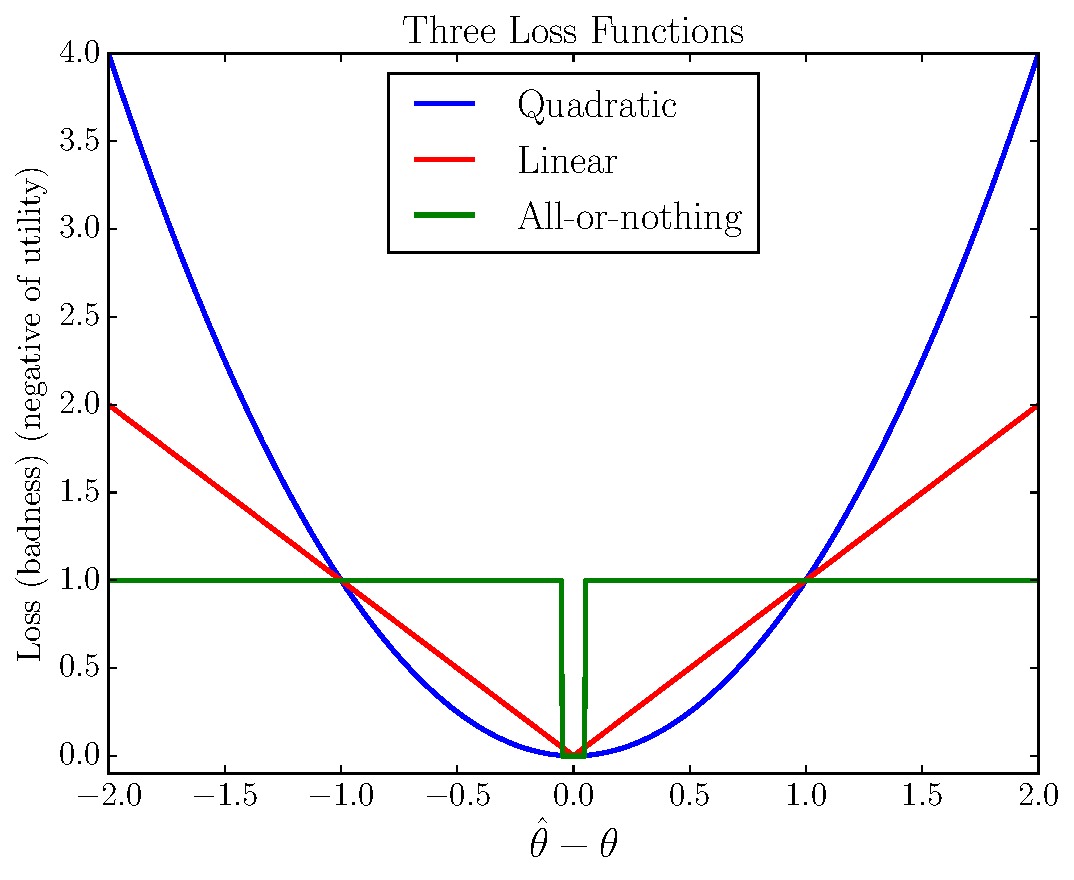
\includegraphics[scale=0.5]{Figures/utility.pdf}
\caption{\it Three kinds of loss function, which measure how bad it is for our
point estimate $\hat{\theta}$ to be different from the true value of the parameter
$\theta$. Note that the all-or-nothing loss has a small amount of width in this
plot, just so that we can clearly see the spike at
$\hat{\theta} - \theta$ = 0.\label{fig:utility}}
\end{center}
\end{figure}

\subsection{Invariance of Decisions}
You may be wondering about the definitions of our loss functions. For example,
we defined the quadratic loss as $(\hat{\theta} - \theta)^2$, but what if we
defined it as $3(\hat{\theta} - \theta)^2 + 5$ instead? Would our
best decision change? Luckily, the answer is no. The decision (estimate) which
minimises the expected value of a loss function $L$ also minimises the expected
value of a different loss function $aL + b$, where $a$ is any positive number
and $b$ is any other number.
For the mathematicians, the optimal decision is invariant under positive affine
transformations of the utility or loss function. Phew!

\subsection{Computing Point Estimates from a Bayes' Box}
We have just discussed three different point estimates, and under what
circumstances we can consider them to be the best possible estimate we could
make. Now, we will look at how to actually obtain the point estimates.
The posterior mean is straightforward. It's the expectation value of the parameter
using the posterior distribution. In R, the code is:
\begin{framed}
\begin{verbatim}
post_mean = sum(theta*post)
\end{verbatim}
\end{framed}
You should also know how to compute this manually from a Bayes' Box, using a
calculator.

The posterior mode is also fairly straightforward. First, we can find the
highest probability in the Bayes' Box. Then we find the corresponding parameter
value.
\begin{framed}
\begin{verbatim}
highest_probability = max(post)
post_mode = theta[post == highest_probability]
\end{verbatim}
\end{framed}
In the case of a tie, {\tt post\_mode} might be a vector, indicating
that there isn't a single mode.

The posterior median is a little harder. We need to find the $\theta$ value
which has 50\% of the probability to the left and 50\% of the probability to the
right. Note that this isn't precisely defined in some cases, particularly with
discrete distributions. For example, if $\theta$ could be 1, 2, or 3, and the
probabilities of these were 0.3, 0.6, and 0.1, then what is the median? It is
not entirely clear. However, if there are a large number of possibilities then
the definition becomes more clear.

To calculate the posterior median in R, we need to use the cumulative distribution
which is defined as $F(t) = P(\theta \leq t)$. If we then find the value of $t$
where $F(t) = 0.5$, we have found the posterior median. This isn't always
possible but we can always find the value of $t$ which makes $F(t)$ very close to
0.5.
To obtain the cumulative distribution
in R you can use the {\tt cumsum} function, which calculates the cumulative sum
of a vector. The posterior vector contains the probabilities of $\theta$ equalling
certain values. If we want the probability that $\theta$ is less than or
equal to a certain value, we sum all the probabilities up to and including that value. The
cumulative sum function achieves this. Here is the code for calculating the
posterior median:
\begin{framed}
\begin{verbatim}
F = cumsum(post)
dist = abs(F - 0.5) # Distance of the F-values from 0.5
post_median = theta[dist == min(dist)]
\end{verbatim}
\end{framed}
Note that this may also produce more than one result. Like the mode, the
posterior median is not always uniquely defined.

\subsection{Computing Point Estimates from Samples}
When we use a Bayes' Box (or the equivalent R commands which represent the
columns of a Bayes' Box as vectors), we end up with a vector of possible parameter
values and another vector containing the posterior distribution.
When we use MCMC and JAGS, the output is different.
We will only have a vector of parameter
values, without corresponding probabilities. The vector of parameter values is
meant to be a random sample of values drawn from the posterior distribution.
It's like saying ``here are a bunch of guesses for the parameter'', and any
region where there are a lot of guesses is considered to be a region with high
probability.

When we have samples instead of an exhaustive list of parameter values and
probabilities, the methods for computing the summaries are different. For a
parameter called $\theta$, the methods for computing the summaries are given
below.

\begin{framed}
\begin{verbatim}
# Posterior mean using samples
post_mean = mean(theta)
# Posterior mode using samples
# post_mode = ??? (this can't be done easily with samples!)
# If you have a really large number of samples,
# visually finding the peak of
# a histogram can work.
# Posterior median using samples
sorted = sort(theta)
post_median = sorted[0.5*length(theta)]
\end{verbatim}
\end{framed}

\section{Credible Intervals}
Credible intervals are another useful kind of summary. They are used to make
statements like ``There is a 95\% probability the parameter is between
100 and 150''. The basic idea is to
use the posterior distribution to find an interval $[a, b]$ such that
\begin{eqnarray}
P(a \leq \theta \leq b | x) &=& \alpha
\end{eqnarray}
where $\alpha$ is some pre-defined probability. 95\% seems to be the
most popular choice. An example of a 95\% credible interval is given in
Figure~\ref{fig:credible_interval}.

\begin{figure}[ht!]
\begin{center}
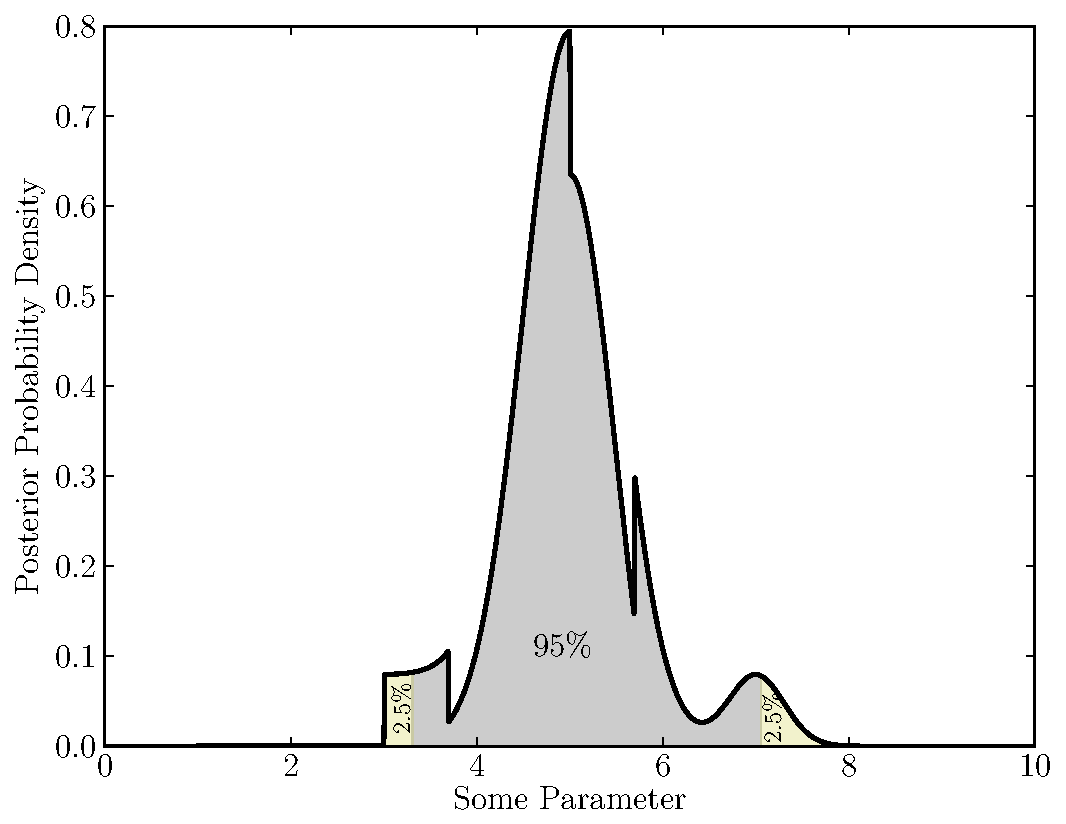
\includegraphics[scale=0.5]{Figures/credible_interval.pdf}
\caption{\it A central 95\% credible interval is defined as an interval that
contains 95\% of the posterior probability, while having 2.5\% of the probability
above the upper limit and 2.5\% of the probability below the lower limit. The
credible interval is formed by finding the edges of the grey region. In this
case the credible interval is $[3.310, 7.056]$.
\label{fig:credible_interval}}
\end{center}
\end{figure}
Note that the interval shown in Figure~\ref{fig:credible_interval} is not the
only possible interval that would contain 95\% of the probability. However, to
make the notion of a credible interval precise, we usually use a {\it central}
credible interval. A central credible interval containing an amount of probability
$\alpha$ will leave $(1-\alpha)/2$ of the probability to its left and
the same amount $(1-\alpha)/2$ of the probability to its right.

\subsection{Computing Credible Intervals from a Bayes' Box}
The method for computing credible intervals is closely related to the method
for computing the posterior median. With the median, we found the value of
$\theta$ which has 50\% of the posterior probability to its left and 50\% to its
right. To find the lower end of a 95\% credible interval, we find the $\theta$
value that has 2.5\% of the probability to its left. To find the upper end we
find the value of $\theta$ that has 2.5\% of the posterior probability to its
right, or 97.5\% to the left.

\subsection{Computing Credible Intervals from Samples}
If you have used MCMC and have obtained random samples from the posterior
distribution, you can find a credible interval in a similar way to how you would
find the posterior median. Again, instead of finding the 0.5 quantile of the
posterior distribution you would find the 0.025 quantile and the 0.975 quantile
(if you wanted a central 95\% credible interval).

\section{Confidence Intervals}
In previous stats courses you have probably come across the concept of a
{\it confidence interval}. A confidence interval is a concept in classical
statistics that is somewhat similar to a credible interval in Bayesian statistics.
When people calculate confidence intervals, they usually want to say they are
95\% sure that the parameter is in that interval,
given the data. This is what Bayesian credible intervals do, but {\it it is not
what classical confidence intervals do}!

Luckily, a lot of the time, the classical and the Bayesian methods for making
intervals will actually give the same interval. But this isn't always the case!
In lectures we will study an example (taken from an Ed Jaynes paper from the
70s)
where the Bayesian credible interval and
the classical confidence interval give completely different results. The result
is shown in Figure~\ref{fig:jaynes}. The key thing to note is the classical
confidence interval lies entirely in a region where we are certain
(from the data) that $\theta$ cannot possibly be!

\begin{figure}[ht!]
\begin{center}
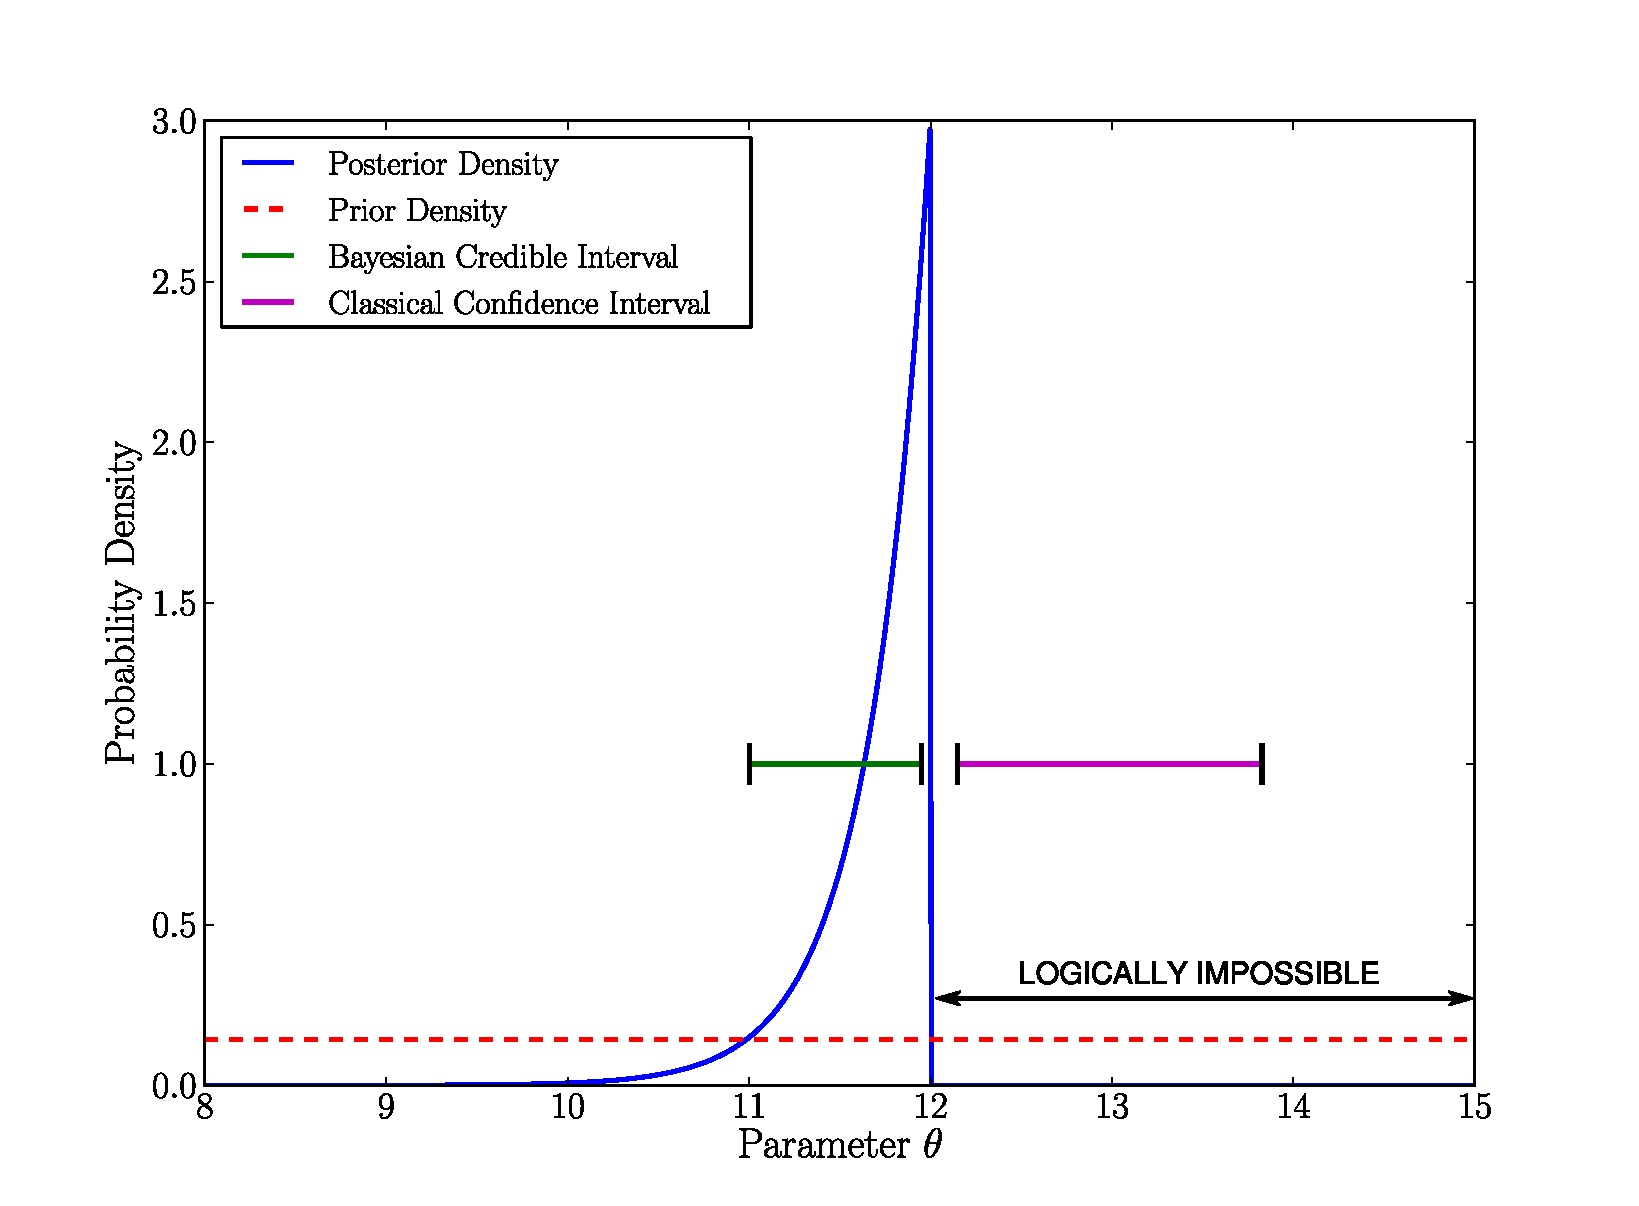
\includegraphics[scale=0.5]{Figures/jaynes.pdf}
\caption{\it An example of a Bayesian credible interval and a frequentist confidence
interval applied to a particular problem where they give different answers.
The posterior distribution in blue shows that the parameter $\theta$ is probably
somewhere between 11 and 12, and values above 12 are completely impossible.
However, the entire frequentist confidence interval lies above $\theta=12$.
\label{fig:jaynes}}
\end{center}
\end{figure}


\chapter{Hypothesis Testing and Model Selection}
Hypothesis testing (also known as model selection, particularly when it is
done using the method in Section~\ref{sec:marginal_likelihood})
is a very important topic that is traditionally considered
a different topic from parameter estimation. However, in Bayesian statistics
we will see that hypothesis testing is basically the same thing as parameter
estimation! The one difference, for us, will be that we will sometimes change
the prior distribution a little bit.

One big advantage of Bayesian statistics is that it {\it unifies}
parameter estimation and hypothesis
testing\footnote{``Unifies'' is a popular word for physicists. It means that
two seemingly different topics are fundamentally the same, or at least closely
related.}. That's good news, because instead of having to
understand two different topics, we only have to understand one!

To see why hypothesis testing is fundamentally the same as parameter estimation,
you only need to
understand how parameter estimation works from a Bayesian point of view, which
we have already studied.
Parameter estimation is nothing more than testing a bunch of hypotheses about
the value of the parameter. For example, $\theta=1$ vs. $\theta=2$ vs. $\theta=3$ and
so on. If we have their posterior probabilities, then we've tested them.

\section{An Example Hypothesis Test}
Suppose we were performing a Bayesian parameter estimation analysis using a
Bayes' Box. Here is an example Bayes' Box with made up numbers:

\begin{table}[h!]
\begin{center}
\begin{tabular}{|c|c|c|c|c|}
\hline
\tt{possible values} & \tt{prior} & \tt{likelihood} & \tt{prior} $\times$ \tt{likelihood} & \tt{posterior}\\
$\theta$ & $p(\theta)$ & $p(x|\theta)$ & $p(\theta)p(x|\theta)$ & $p(\theta|x)$\\
\hline
1.5 & 0.25 & 0.2 & 0.05 & 0.1\\
2.0 & 0.25 & 0.4 & 0.1 & 0.2\\
2.5 & 0.25 & 0.6 & 0.15 & 0.3\\
3.0 & 0.25 & 0.8 & 0.2 & 0.4\\
\hline
Totals & 1 & & 0.5 & 1\\
\hline
\end{tabular}
\end{center}
\end{table}
Suppose we wanted to test the following two hypotheses about the parameter $\theta$.
The first hypothesis $H_0$ is a ``null hypothesis'', and the second hypothesis,
$H_1$, is an ``alternative hypothesis''.
\begin{eqnarray}
H_0: && \theta = 2\\
H_1: && \theta \neq 2
\end{eqnarray}
In classical statistics, if you saw a question phrased in this way, you would
need to come up with a {\it test statistic}
and then calculate a {\it p-value}, which tries to say something about whether
the value of the test statistic would be considered extreme, under the
assumption that $H_0$ is true.
In Bayesian statistics, the only thing we need to do is calculate
the posterior probability of $H_0$ and the posterior probability of $H_1$.
The posterior probability of $H_0$ is given by:
\begin{eqnarray}
P(H_0|x) &=& P(\theta = 2|x)\\
&=& 0.2
\end{eqnarray}
All we did here was look up the appropriate number in the Bayes' Box! The
posterior probability of $H_1$ is only slightly harder (but still easy)
to calculate: $H_1$ will
be true if $\theta$ takes any value other than 2. Therefore, the posterior
probability of $H_1$ is
\begin{eqnarray}
P(H_1|x) &=& P(\theta = 1.5 \textbf{ or } \theta = 2.5 \textbf{ or } \theta = 3|x)\\
&=& P(\theta = 1.5|x) + P(\theta = 2.5|x) + P(\theta = 3|x)\\
&=& 0.1 + 0.3 + 0.4\\
&=& 0.8.
\end{eqnarray}
Here we used the fact that everything in a Bayes' Box is mutually exclusive
(only one of the hypotheses is true) so we could add the probabilities.
Alternatively, you could have just noticed that $H_1$ is true if $H_0$ is false.
So $P(H_0|x) + P(H_1|x) = 1$, which implies $P(H_1|x) = 1 - P(H_0|x)$.

\section{The ``Testing'' Prior}
Here we will study a hypothesis testing example that involves a null and an
alternative hypothesis. Since the bus example has been used a lot, we will now
switch over to a different example.

Suppose it is known that the mean systolic blood pressure
in the general population is 120 mm Hg, with a standard deviation of
15 mm Hg (millimetres of mercury is an
old fashioned unit for pressure, even though it sounds like a unit of length).
A new drug is developed that may
be helpful in reducing blood pressure. A sample of 100 people
(who can be considered representative of the general population)
are given the drug, and their systolic blood pressure is measured. This results
in 100 blood pressure measurements $\{x_1, x_2, ..., x_{100}\}$, which will be
our data.

We are interested in whether the drug works. Let $\mu$ be the mean systolic
blood pressure
that would apply in the general population if everyone was taking the
drug. Our goal is to infer the value of $\mu$ from the data. In classical
statistics, this is sometimes phrased as a hypothesis test between the two
competing hypotheses. We will not be concerned with the possibility that the
drug has the opposite effect to what is intended.
\begin{equation}
\begin{array}{ll}
H_0: & \mu = 120 \textnormal{ (the drug does nothing)}\\
H_1: & \mu < 120 \textnormal{ (the drug reduces blood pressure)}
\end{array}
\end{equation}
Suppose the mean of all the data values was
\begin{eqnarray}
\bar{x} &=& \frac{1}{N} \sum_{i=1}^{100} x_i\\
&=& 115.9.
\end{eqnarray}
Does this data provide evidence against $H_0$ and in favour of $H_1$? In
classical statistics this question would be addressed using a {\it p-value}.
The p-value would be the probability of getting a result this extreme or
a result more extreme than what is observed, assuming that the ``null hypothesis''
is true. That is,
\begin{eqnarray}
\textnormal{p-value} = P(\bar{x} \leq 115.9 | H_0).
\end{eqnarray}
In case you're curious, the p-value in this case is 0.0031, which is usually
taken to mean that there is fairly strong evidence against $H_0$ and in favour
of $H_1$. To calculate the p-value I had to assume that the probability distribution
for the data values $\{x_1, x_2, ..., x_{100}\}$ was a normal distribution
with a known standard deviation of $\sigma=15$, and
that they were independent:
\begin{eqnarray}
x_i \sim \mathcal{N}(\mu, \sigma^2). \label{eq:normal}
\end{eqnarray}

In Bayesian statistics, p-values are not used. Instead, we should think of this
as a parameter estimation problem. We can state a set of hypotheses about the
value of $\mu$, and then choose a prior distribution, update to a posterior
distribution, etc. Then our result will be the posterior probability of the
null hypothesis, $P(H_0 | \{x_1, ..., x_{100}\}) = P(\mu = 120 | \{x_1, ..., x_{100}\})$.
This is helpful because the posterior probability of the null hypothesis is
exactly what we want. It is a description of how plausible the null hypothesis
is given the data. It is not some other probability that isn't really relevant.
We can also get the posterior probability of $H_1$ by summing the posterior
probabilities for all other values of $\mu$ apart from 120, or by using
$P(H_1 | \{x_1,...,x_{100}\}) = 1 - P(H_0 | \{x_1,...,x_{100}\})$.

There is only one minor tweak we need to make to make Bayesian inference an
appropriate framework for solving this problem. When the null and alternative
hypotheses are written like we wrote them above, it implies that the value of $\mu$
that we are calling the ``null hypothesis'' is a {\it special value that is
especially plausible}. To take this into account in our Bayesian analysis we
need to make sure the prior distribution recognises there is a special
value of the parameter that we think is extra plausible. When we do this, we
will call it a {\it testing prior}. An example of a testing prior and the
resulting Bayes' Box for
the blood pressure problem is given in Table~\ref{tab:testing_prior}.
The R code for calculating these results is given below.

\begin{minted}[mathescape,
               numbersep=5pt,
               gobble=0,
               frame=single,
               framesep=2mm, fontsize=\small]{r}
# Parameter values
mu = seq(110, 120)

# Make the testing prior
prior = rep(0.5/10, 11)
prior[11] = 0.5

# Compute the likelihood for the 100 data points.
# The numbers get close to 0, so logs would be useful
lik = 1
# Use a for loop to loop over all data values
# and multiply the likelihoods
for(i in 1:100)
{
    lik = lik*dnorm(x[i], mean=mu, sd=15)
}

# Rescale the likelihood for readability
lik = lik/max(lik)*1000

# Calculate the posterior
h = prior*lik
post = h/sum(h)

# The null hypothesis
post[11]
\end{minted}


\begin{table}[ht!]
\begin{center}
\begin{tabular}{|c|c|c|c|c|}
\hline
\tt{possible values} & \tt{prior} & \tt{likelihood} & \tt{prior} $\times$ \tt{likelihood} & \tt{posterior}\\
$\mu$ & $p(\mu)$ & $p(\{x_1, ..., x_{100}\}|\mu)$ & $p(\mu)p(\{x_1, ..., x_{100}\}|\mu)$ & $p(\mu|\{x_1, ..., x_{100}\})$\\
\hline
110 & 0.05 & 0.44	& 0.02 & 0.0001\\
111 & 0.05 & 4.83	& 0.24 & 0.0012\\
112 & 0.05 & 34.12	& 1.71 & 0.0086\\
113 & 0.05 & 154.64	& 7.73 & 0.0389\\
114 & 0.05 & 449.33	& 22.47 & 0.1129\\
115 & 0.05 & 837.13	& 41.86 & 0.2103\\
116 & 0.05 & 1000.00    & 50.00 & 0.2512\\
117 & 0.05 & 756.93	& 38.30 & 0.1924\\
118 & 0.05 & 376.15	& 18.81 & 0.0945\\
119 & 0.05 & 118.44	& 5.92 & 0.0298\\
{\bf 120} & {\bf 0.5}   & {\bf 23.91} & {\bf 11.96} & {\bf 0.0601}\\
\hline
Totals & 1 & & 199.01 & 1\\
\hline
\end{tabular}
\caption{\it An example of a testing prior for the blood pressure problem. We
give more prior probability to the special value $\mu=120$ because it is
particularly plausible. For readability I have rescaled the likelihoods so that
the maximum is 1000. Note that the posterior probability of $H_0$ can simply
be read off the table.
\label{tab:testing_prior}}
\end{center}
\end{table}

The conclusion of our Bayesian hypothesis test is that the posterior probability
of $H_0$ is 0.0601. Recall that the classical p-value was 0.0031. These numbers
are very different, and there is no reason why they should be similar. The
p-value might imply that the evidence is overwhelming (if you are not experienced
at interpreting p-values), but the posterior probability still says there's a
6\% chance the drug does nothing.

Note that the calculation of the posterior distribution uses {\it all} of the
data values, rather than reducing the whole data set down to a single number
(the sample mean $\bar{x}$). In this particular example, reducing the whole
dataset to a single number is harmless\footnote{In this problem, the sample mean
is a ``sufficient statistic''. In this
particular problem, throwing away information has no
consequences!}. But in different situations (e.g. if your sampling distribution
or likelihood was based on the heavy-tailed Cauchy distribution instead of a normal
distribution), reducing an entire data set to a single ``test statistic'' can
be extremely wasteful!

Note also that there were some fairly arbitrary decisions made in choosing our
testing prior. We decided not to allow $\mu > 120$, but the analysis could
also have allowed for that. The discrete approximation was fairly coarse. Finally, we
assumed $\mu$ couldn't be lower than 110, and had a uniform prior for all
$\mu$ values apart from 120. Some of these assumptions can and should be
questioned when applying Bayesian hypothesis testing in practice.
In Figure~\ref{fig:testing_priors}, there are three possible ideas for what
the prior should be in the blood pressure question. They may all seem reasonable in this situation.
Prior 1 is basically the same as the prior in our Bayes' Box, although it goes
down to $\mu=100$ and divides the possible $\mu$ values more finely. This prior
says the null has a 50\% probability, and if $\mu$ is not equal to 120, then it
could be anything.
Prior 2
is similar, but has only 30\% of the prior probability on the null hypothesis,
instead of 50\%,
and the shape of the prior is non-uniform for the lower values of $\mu$.
This is like saying ``$\mu$ could be precisely 120, and if it's not precisely
120, then it is probably at least {\it close} to 120''. In a lot of hypothesis
testing situations this would be a more accurate description of our prior
beliefs than Prior 1.
Prior 3 isn't really a testing prior at all (it doesn't have a spike), but is
just a bell-shaped prior. This is like saying ``Alright, I would never believe
$\mu$ is {\it exactly} 120, but I think there's a reasonable chance it's {\it
close} to 120. Often, it would be nonsense to think the null hypothesis
is perfectly true, to an arbitrary level of accuracy. Something like Prior 3
would be more appropriate.
These three priors would all give different results, and the appropriate choice
depends on the individual problem you are solving. 

\begin{framed}
{\bf Remember, if the conclusions depend sensitively on the choice of the
prior distribution, then that is an important finding. You either need to be
really careful about choosing your prior, or you need more data.}
\end{framed}

\begin{figure}[ht!]
\begin{center}
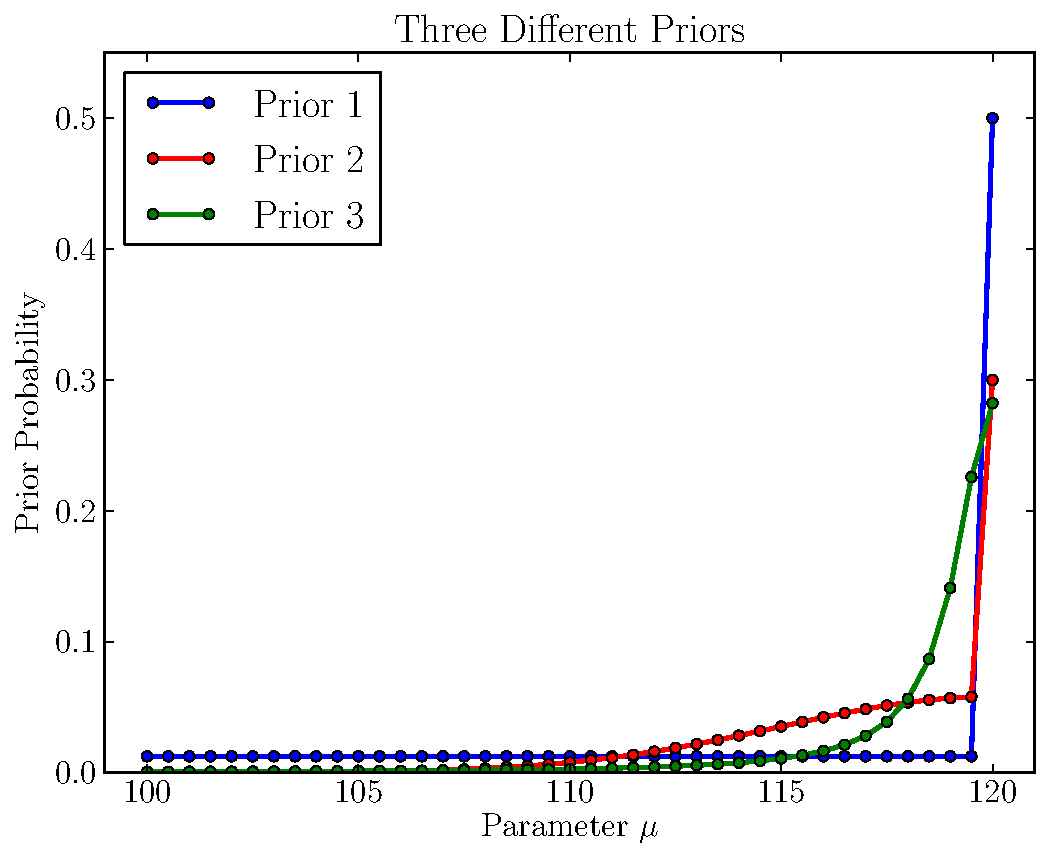
\includegraphics[scale=0.6]{Figures/testing_priors.pdf}
\caption{\it Three possible priors we could use for the blood pressure question.
All may seem ``reasonable'', and the choice can affect the results (quite
significantly in some cases). Care should be taken when choosing the prior
in hypothesis testing problems.
\label{fig:testing_priors}}
\end{center}
\end{figure}


\section{Some Terminology}
There is some alternative terminology that is widely used and is particularly
popular in Bayesian hypothesis testing (aka model selection) problems. Suppose
there were two hypotheses $H_1$ and $H_2$, and some data $x$. Now, $H_1$ and
$H_2$ might be a null and alternative hypothesis, or they might be two
particular values of the parameter, or something else. Two repetitions of Bayes' rule
for these two hypotheses are:
\begin{eqnarray}
P(H_1 | x) &=& \frac{P(H_1)p(x|H_1)}{p(x)}\\
P(H_2 | x) &=& \frac{P(H_2)p(x|H_2)}{p(x)}
\end{eqnarray}
These could also be written in words:
\begin{eqnarray}
\textnormal{posterior} &=& \frac{\textnormal{prior}\times\textnormal{likelihood}}{\textnormal{marginal likelihood}}
\end{eqnarray}

Dividing these two equations gives the {\it odds form} of Bayes' rule, which
deals with ratios of probabilities instead of probabilities themselves.
\begin{eqnarray}
\frac{P(H_1 | x)}{P(H_2|x)} &=& \frac{P(H_1)}{P(H_2)} \times
\frac{p(x|H_1)}{p(x|H_2)}\label{eq:odds_form}
\end{eqnarray}
In words, this can be written as:
\begin{eqnarray}
\textnormal{posterior odds} = \textnormal{prior odds}
\times
\textnormal{bayes factor}
\end{eqnarray}
Sometimes people talk about odds (or odds ratios, which are the same thing)
and Bayes Factors instead of about prior and
posterior probabilities. The odds tell us how plausible $H_1$ is compared to
$H_2$. For example, a posterior odds ratio of 5 means $H_1$ is 5 times as plausible
as $H_2$. Of course, odds can be greater than 1 even though probabilities
cannot be. The Bayes Factor is the ratio of the likelihoods. Results are often
quoted as Bayes Factors because that's the part of the equation where the
data is important. If you say ``The Bayes Factor for $H_1$ over $H_2$ was 10'',
then whoever you're talking to is free to apply whatever prior odds they like,
whereas if you state the posterior odds then people may wonder what your prior
odds were.

\section{Hypothesis Testing and the Marginal Likelihood}\label{sec:marginal_likelihood}
The Bayes' factor in Equation~\ref{eq:odds_form} is the ratio of likelihoods
for two hypotheses $H_1$ and $H_2$. If we wanted to calculate the Bayes Factor
for $H_0$ and $H_1$ in the blood pressure example, we could easily get the likelihood
for $H_0$ (it's right there in the Bayes' Box). But how would we get $p(x|H_1)$,
which needs to be a single number? $H_1$ is the statement $\mu = 100$ {\bf or}
$\mu = 111$ {\bf or} $\mu = 112$ and so on up to $\mu = 119$.

Imagine we had left $\mu=120$ out of our Bayes' Box and just done parameter
estimation within the context of $H_1$ (i.e. assuming, for argument's sake,
that $H_1$ is true). This would involve a {\it reduced} Bayes' Box with one
less row in it. We would end up getting some marginal likelihood
$p(x) = \sum p(\theta)p(x|\theta)$.
The key is to realise that since we are assuming $H_1$ throughout, the
marginal likelihood is really $p(x|H_1) = \sum p(\theta|H_1)p(x|\theta, H_1)$,
which is exactly the thing we need to calculate the Bayes Factor!

All of this implies
there are two mathematically equivalent ways of doing Bayesian hypothesis testing,
or model selection. One is to make a big model that includes both the null and
the alternative hypothesis. The Bayes' Box with a testing prior accomplishes this.
In most cases this is the most convenient way to do the calculations.

The other way is to do the two analyses separately. First, do parameter estimation
within the context of $H_1$. Then, do parameter estimation within the context
of $H_2$. Then, use the marginal likelihoods as if they were likelihoods, to
compare $H_1$ vs. $H_2$. This second way of calculating Bayes Factors is
most useful when the two analyses were actually done separately by different
people.

\section{Analytic Solution}

Let's make the prior for $\mu$, conditional on $H_1$, a normal distribution
centered at $m$ with a standard deviation of $s$.

\begin{eqnarray}
p(\mu | H_1) &=& \frac{1}{s\sqrt{2\pi}}\exp
\left[-\frac{1}{2s^2}\left(\mu - m\right)^2\right]
\end{eqnarray}

Using Bayes' rule, the posterior is proportional to the prior multiplied by
the likelihood. This is all conditional on $H_1$, which we should remember
to put in the right hand side of the ``given'' sign in all of our terms:

\begin{eqnarray}
p(\mu | x, H_1) &\propto& p(\mu | H_1)p(x | \mu, H_1) \\
&\propto&
\frac{1}{s\sqrt{2\pi}}\exp
\left[-\frac{1}{2s^2}\left(\mu - m\right)^2\right]
\times
\prod_{i=1}^N \frac{1}{\sigma\sqrt{2\pi}}
\exp
\left[-\frac{1}{2\sigma^2}\left(x_i - \mu\right)^2\right]
\end{eqnarray}


\chapter{Markov Chain Monte Carlo}
\section{Monte Carlo}
Monte Carlo is a general term for computational techniques that use random
numbers.
Monte Carlo can be used in classical and Bayesian statistics, and a special kind
called Markov Chain Monte Carlo (MCMC) was one of the main reasons
for the revival of Bayesian statistics in the second half of the 20th century.
Before MCMC became popular, one of the major drawbacks of the Bayesian approach
was that the calculations were too hard. 

\subsection{Summaries}
So far, we have represented our probability distributions (prior and posterior)
in a computer by using a vector of possible parameter values and a corresponding
vector of probabilities. For example, suppose we had a single parameter $\theta$
and we had worked out the posterior distribution by using a Bayes' Box. This
will have given us a vector {\tt theta} of possible $\theta$ values and a corresponding
vector {\tt post} containing the posterior probabilities. Well, one thing we could
do is plot the posterior distribution:
\begin{verbatim}
plot(theta, post, xlab="Theta", ylab="Posterior Probability")
\end{verbatim}
This would make a plot something like the following:

\begin{figure}[ht!]
\begin{center}
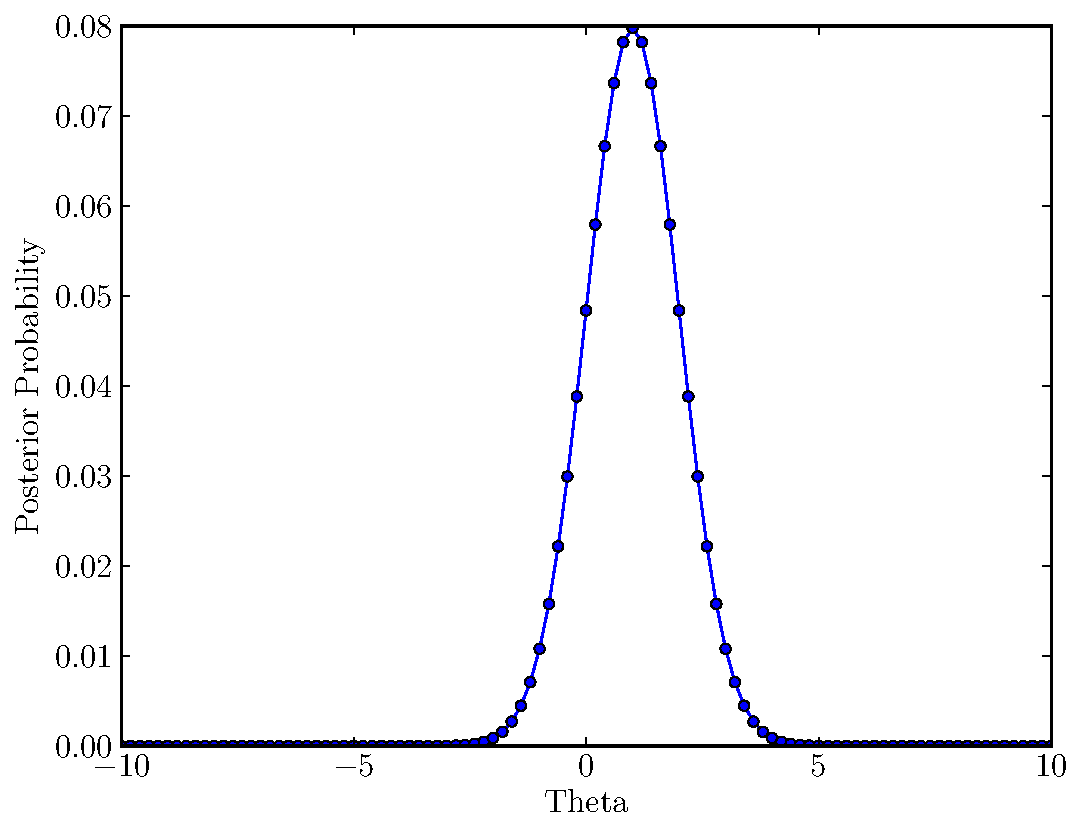
\includegraphics[scale=0.5]{Figures/normal.pdf}
\caption{\it A posterior distribution can be represented in a computer by a discrete
set of possible parameter values, and the corresponding probabilities.\label{fig:normal}}
\end{center}
\end{figure}

If we wanted to obtain some summaries, we could do it like so:
\begin{verbatim}
post_mean = sum(theta*post)
post_sd = sqrt(sum(theta^2*post) - post_mean^2)
\end{verbatim}

However,
there is an alternative way of representing this posterior distribution in a
computer. It may not be immediately obvious why this is a good idea,
because there is nothing wrong with the tried and true method we have used
so far. But this second method has the advantage that it continues to
work well on much bigger problems, such as when we have more than one parameter.
With more than one parameter, the `vector of possible solutions'' approach
can fail very dramatically.

Our new way of representing a probability distribution in a computer will be
via {\it Monte Carlo} samples.
Instead of having two vectors (one of $\theta$ values and one of the
corresponding probabilities),
imagine we had some method to compute a random sample of $\theta$ values, drawn
from the posterior distribution in Figure~\ref{fig:normal}.
There would only be one vector {\tt theta}. So how would we
know that there is greater probability around $\theta=1$? Well, {\it more elements
of the {\tt theta} vector would be near 1}.
Instead of carrying around a second vector of
probabilities, we simply let the fact that there are lots of points in certain
regions tell us that those regions are more probable. Say our vector of random
samples was called {\tt theta}. Then we could look at the posterior distribution
by plotting a histogram of samples:
\begin{verbatim}
hist(theta, breaks=100)
\end{verbatim}
The histogram would look something like this:

\begin{figure}[ht!]
\begin{center}
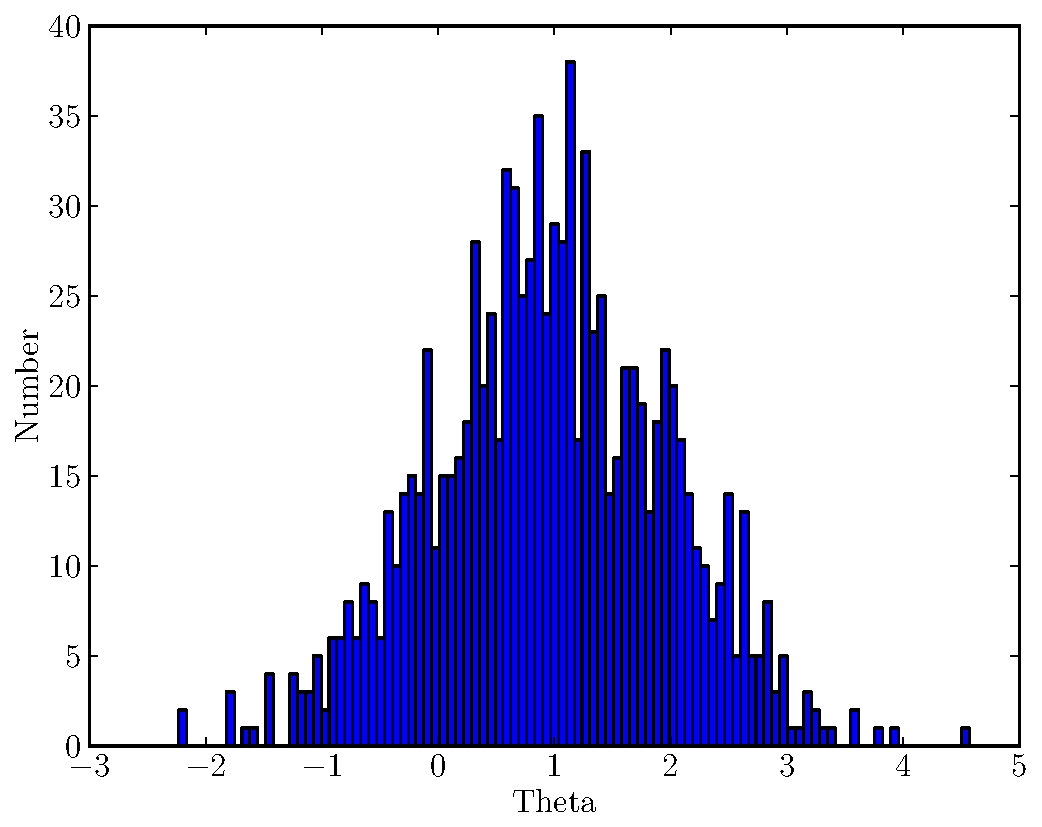
\includegraphics[scale=0.5]{Figures/normal2.pdf}
\caption{\it The posterior distribution for a parameter $\theta$ can also be
represented by a random sample of $\theta$ values drawn from the posterior
distribution. The fact that some $\theta$ values are more probable than others
is encoded by the fact that certain values appear more frequently in the sample.
\label{fig:normal2}}
\end{center}
\end{figure}

We could also get our summaries, but the code looks different
(it's actually easier!):
\begin{verbatim}
post_mean = mean(theta)
post_sd = sd(theta)
\end{verbatim}
Because of the randomness involved in generating the {\tt theta} values,
the summaries aren't exact. For example, I know that the actual posterior mean
and standard deviation in this example were both 1, but the values obtained
from the Monte Carlo samples were 0.9604 and 1.0008 respectively. This doesn't
matter much though, because the conclusions about $\theta$ are that it is probably
somewhere around 1 with an uncertainty of about 1, and the error introduced by
using random samples are much smaller than the amount of uncertainty inherent
in the posterior distribution itself. For example, if I summarised the posterior
distribution by saying $\theta = 0.9604 \pm 1.0008$, for almost all practical
purposes the conclusion is exactly the same as the true version of the summaries
$\theta = 1 \pm 1$.

In this discussion we haven't answered the question of how to actually generate
random samples of $\theta$ from the posterior distribution. This is the job
of Markov Chain Monte Carlo.

\begin{framed}
{\bf
The purpose of Markov Chain Monte Carlo is to generate random samples of
parameter values drawn from the posterior distribution. This makes it very easy
to compute summaries even if you have more than one unknown parameter.}
\end{framed}

\section{Multiple Parameters}
MCMC becomes extremely useful when we begin to look at Bayesian models involving
more than one unknown parameter. 
Having posterior samples makes the process of {\it marginalisation}
much easier. Imagine we wanted to infer $a$ and $b$ from
data $x$. Bayes' rule (parameter estimation version) would give us the posterior
distribution:
\begin{eqnarray}
p(a, b | x) \propto p(a, b)p(x|a,b)
\end{eqnarray}

However, what if you didn't really care about the value of $b$ but
only really wanted to measure $a$. The terminology for this is that $b$ is a
{\it nuisance parameter}: you need it to define the model, but ultimately you
are not really interested in knowing its value.
What you need in this case is the
{\it marginal} posterior distribution for $a$ (that is, the posterior
distribution for $a$ on its own, not the joint distribution with $b$).
This can be obtained using the sum rule. The result is:
\begin{eqnarray}
p(a | x) &=& \int_b p(a, b|x) \, db
\end{eqnarray}
or
\begin{eqnarray}
p(a | x) &=& \sum_{b} p(a, b|x)
\end{eqnarray}
depending on whether the possible $b$ values are continuous or discrete.
Before MCMC, these integrals or sums usually couldn't be done without making
certain choices purely for mathematical convenience (e.g. choosing the prior
to be a certain kind of distribution, not because it is a good model of your
prior beliefs, but only because the maths works out neatly).

Samples of parameter values drawn from the posterior distribution
(achieved using MCMC) make this hard problem much easier. We no longer need
to worry about mathematical convenience.
See Figure~\ref{fig:marginalisation} for an example showing how Monte Carlo
sampling makes marginalisation trivial.

\begin{figure}[ht!]
\begin{center}
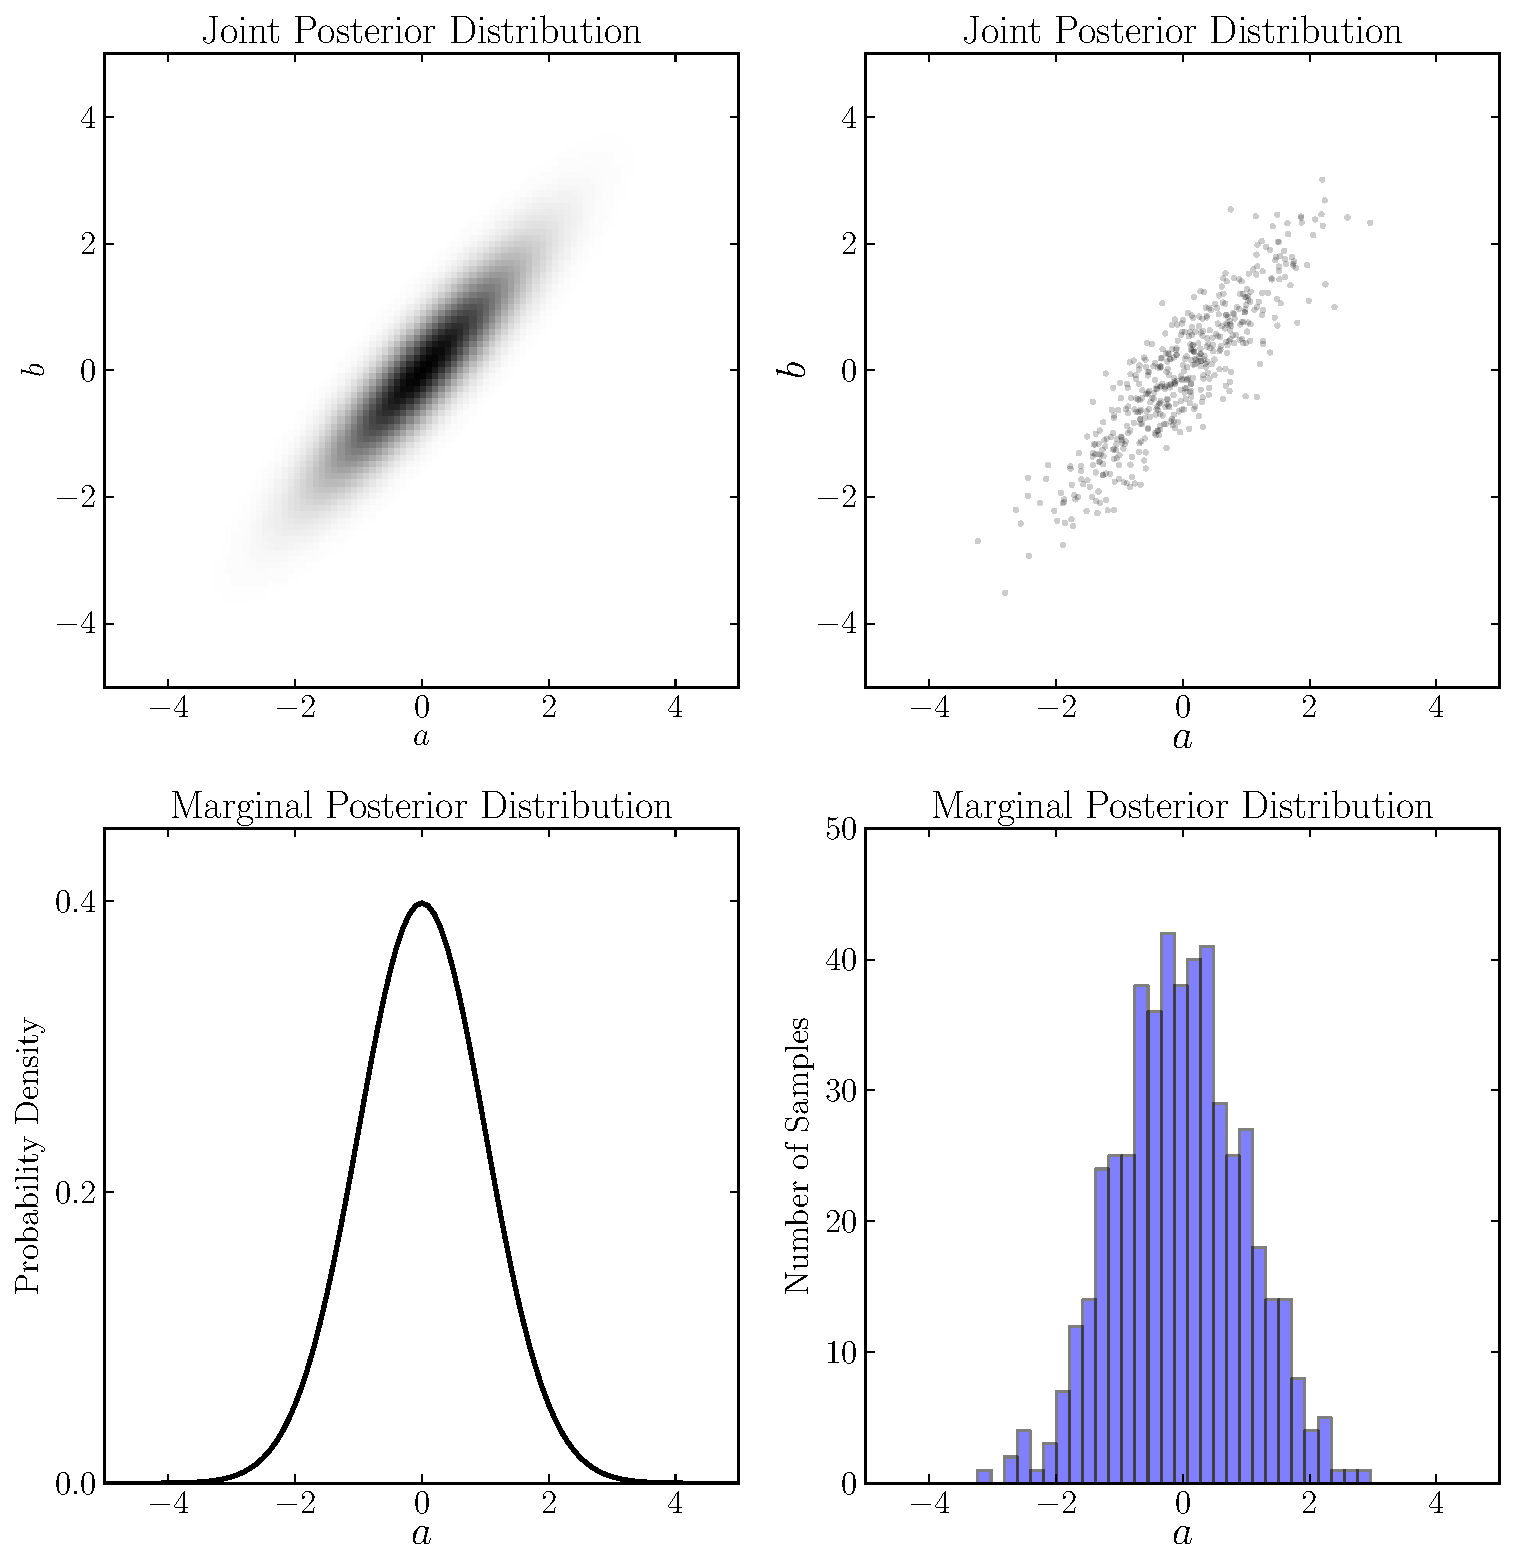
\includegraphics[scale=0.5]{Figures/marginalisation.pdf}
\caption{\it An example of a posterior distribution for two parameters, $a$ and
$b$. The left panels show the joint posterior distribution (which has a
correlation) and the marginal posterior distribution for $a$, obtained by
integrating over all the possible $b$ values. The top right panel contains
random samples
(points) drawn from the posterior distribution for $a$ and $b$.
All you need to do to get the
marginal distribution for $a$ (lower right panel) is ignore the $b$-values of
the points!
\label{fig:marginalisation}}
\end{center}
\end{figure}


\section{The Metropolis Algorithm}
The Metropolis algorithm is the most basic MCMC method.
The ideas behind it are fairly simple, yet Metropolis forms the basis of a large
number of more advanced MCMC methods. In STATS 331 we will study the basic ideas
behind how the Metropolis algorithm works. We will look at a small amount of R code
that implements the Metropolis algorithm, but for solving practical problems
it is more convenient to use the JAGS program\footnote{JAGS uses a number
of MCMC methods internally, including Metropolis, ``Gibbs Sampling'', and
``Slice Sampling'', which we will not study in this course.}.

The Metropolis algorithm was invented in the 1950s by physicists
(including Nicholas Metropolis, for whom the algorithm is named), who used it
to do calculations in the field of statistical mechanics. This intriguing field
focuses on calculating the macroscopic (large scale) properties of matter from
knowledge of the small-scale properties: for example, knowing that water is
H$_2$O, you could use statistical mechanics to figure out that if you have a lot
of water molecules, it will freeze at 0 degrees Celsius and boil at 100 degrees
Celsius.

It took
many decades before people started to realise that the Metropolis algorithm was useful in Bayesian
statistics as well. Even though the Bayesian approached seemed very elegant and
useful to many people, it could always be criticised on the basis that, in order
to implement it on practical problems, you usually had to do difficult or
impossible integrals (to summarise the posterior, or to get rid of nuisance
parameters). MCMC changed all that, and is one of the reasons for the
explosion in the popularity of Bayesian statistics beginning in the 1990s.

\begin{framed}
{\bf
The basic idea of MCMC is that we want a method that will travel between
different possible states (such as the possible hypotheses/parameter values in
a Bayesian analysis), and has the property that the amount of time spent in
any particular state is proportional to the posterior probability of that state.}
\end{framed}

\begin{figure}[ht!]
\begin{center}
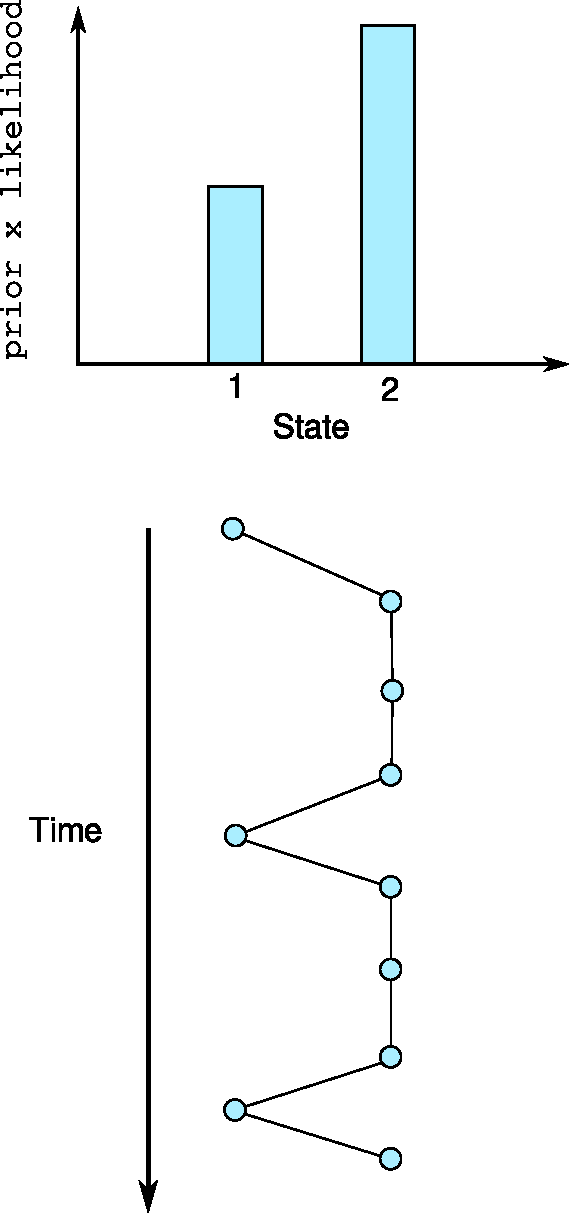
\includegraphics[scale=0.65]{Figures/mcmc.pdf}
\caption{\it An illustration of the basic idea behind MCMC. Imagine we had a
Bayes' Box with two possible states, and we knew the
{\tt prior $\times$ likelihood} values. The amount of time the MCMC program will
spend in each state is proportional to the posterior probability of the state.
In this example, the MCMC algorithm was in State 1 three times and in State 2
seven times. Using this, we could estimate the posterior probability of State 2
as being 0.7. This estimate would become more accurate if we ran the MCMC for
more iterations.\label{fig:mcmc}}
\end{center}
\end{figure}

\subsection{Metropolis, Stated}
The Metropolis algorithm is given below. The first thing to do is start
{\it somewhere} in the ``parameter space'' (set of possible parameter values).
You then
{\it propose} to move somewhere else. There is an acceptance probability $\alpha$
that determines whether to accept the proposal. If the proposal is better
($h$, the prior times likelihood value is higher), then you accept it. If the
proposal is worse, you can also accept it, but the probability of accepting is
then $h'/h$ (e.g. if the proposed point is 1/3 as good as the current point, the
acceptance probability is 1/3).

The Metropolis algorithm works by making transitions towards low probability
states rare, but transitions towards high probability states are common, because
of the acceptance probability. It is hard to move into an improbable state, so
not much time will be spent there.

\begin{framed}
\begin{itemize}
\item Start in some state $\theta$
\item Generate a ``proposal'' state $\theta'$ from a {\it proposal distribution}
\item With probability $\alpha = \textnormal{min}(1, h'/h)$, replace the current
state with the proposed state
\item Repeat
\end{itemize}
\end{framed}

\section{A Two State Problem}
We will now study how the Metropolis algorithm would work on a very simple
example, namely the two-ball problem from the beginning of the notes. There
were two hypotheses and the posterior probabilities were $1/3$ and $2/3$.
It is important to note that MCMC is not actually needed for a problem this
simple, but it is a good test case to see precisely how an MCMC algorithm works.
This means we'll discuss a small amount of Markov chain theory.
However, when we solve real data analysis problems with JAGS,
we won't have to think too
much about how the MCMC works.

Let's
call the less probable hypothesis ``State 1'' and the more probable hypothesis
``State 2'' for the purposes of this section.
What we need is a Markov process that will spend 1/3 of the time in State 1 and
2/3 of the time in State 2. The Metropolis algorithm described above will
do what we need. The main thing we need to compute are the acceptance probabilities
$\alpha_{ij}$ for a proposed transition from state $i$ to state $j$ where
$i, j \in \{1, 2\}$.
The acceptance probability $\alpha$ for a proposed move from state $i$ to
state $j$ is given by:
\begin{eqnarray}
\alpha_{ij} = \textnormal{min}\left(1, \frac{h_j}{h_i}\right)
\end{eqnarray}
where $h_i$ and $h_j$ are proportional to the posterior probabilities of
states $i$ and $j$ respectively. This means that if the proposal is to move
to an equal or better (higher posterior probability)
state ($h_j \geq h_i$) then the acceptance probability is 1.
If the proposal is to move to a less probable state then the acceptance probability
is $h_j/h_i$, the ratio of the two posterior probabilities\footnote{Note that
this algorithm can be used even if the marginal likelihood is unknown, because
only ratios of posterior probabilities are needed. This is useful because the
marginal likelihood is sometimes very hard to calculate in multi-parameter
problems.}.

The transition probability is the probability
of being in state $j$ at the next iteration given that you are in state $i$
at the current iteration. The transition probability is given by the product
rule:
\begin{eqnarray}
p_{ij} = q_j \alpha_{ij}\label{eq:transition}
\end{eqnarray}
for $i \neq j$.
The transition matrix of the Markov chain is a matrix with all the different
$p_{ij}$ values in it:
\begin{eqnarray}
\mathbf{P} &=&
\left[
\begin{array}{cc}
p_{11} & p_{12}\\
p_{21} & p_{22}
\end{array}
\right]
\end{eqnarray}
In our particular case, we can work out the off-diagonal elements of
$\mathbf{P}$ using Equation~\ref{eq:transition}:
\begin{eqnarray}
\mathbf{P}
&=&
\left[
\begin{array}{cc}
 & \frac{1}{2} \times 1\\
\frac{1}{2}\times\frac{1}{2} & 
\end{array}
\right]
\end{eqnarray}
The diagonal elements can be found by knowing that the rows of $\mathbf{P}$ must
sum to 1. We must be in {\it some} state at the next iteration. Therefore the
transition matrix of our Markov chain on this two-state problem is:
\begin{eqnarray}
\mathbf{P}
&=&
\left[
\begin{array}{cc}
\frac{1}{2} & \frac{1}{2}\\
\frac{1}{4} & \frac{3}{4}
\end{array}
\right]
\end{eqnarray}

A Markov chain with a small number of possible states can be represented
graphically using a {\it transition diagram}, as in
Figure~\ref{fig:transitions}.

\begin{figure}[ht!]
\begin{center}
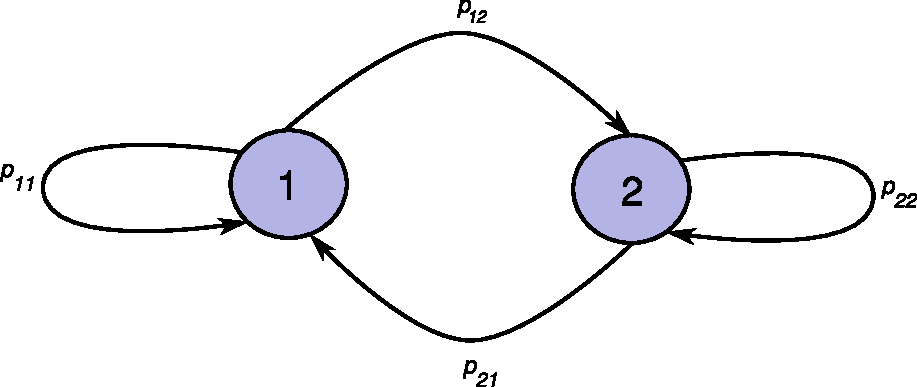
\includegraphics[scale=0.65]{Figures/transitions.pdf}
\caption{\it A transition diagram for a Markov Chain with two possible states.
The states (which correspond to hypotheses in Bayesian inference) are drawn
as circles labelled ``1'' and ``2''. When the algorithm is in a particular state
(e.g. State 1) there is a certain probability $p_{11}$ that it will be in State
1 again at the next iteration, and another probability $p_{12}$ that it will
move to State 2. MCMC works by making it easy to move into states with high
posterior probability, and hard to move out of them.
\label{fig:transitions}}
\end{center}
\end{figure}


In class we will do ``Tactile MCMC'', which is an implementation of the
Metropolis algorithm using coins and dice instead of the random number generators
provided in computer software such as R.

\chapter{Using JAGS}
JAGS stands for ``Just Another Gibbs Sampler''. JAGS is a computer program that
allows the user
to implement Markov Chain Monte Carlo (MCMC) on fairly complicated problems
very quickly. The ``Gibbs Sampling'' mentioned in the name of JAGS
is a particular MCMC technique that is beyond the
scope of this course: however, it is not so different from the Metropolis-Hastings
method that we do study in this course. If you are faced with a statistics
problem which you would like to solve in a Bayesian way, JAGS makes it very
straightforward to implement a Bayesian model. Essentially, you just need to tell
JAGS the following things:
\begin{itemize}
\item The names of your unknown parameter(s), and their prior distributions
\item The likelihood
\end{itemize}
Then we simply load in the data and let it go! JAGS will run MCMC, automatically
choosing an appropriate starting point based on your prior,
and moving the parameter
values around so the posterior distribution is well sampled.
In this chapter we will see how to use JAGS with a simple example, and we will
see some more features of JAGS when we come to study more complex examples.
There are some more advanced features of JAGS that we will not use in this
course.

JAGS is not the first program of its kind, and it is related to many other
available programs.
Starting in the late 1980s, a program called BUGS (Bayesian inference Using
Gibbs Sampling) was developed, and this evolved into the program WinBUGS. These
programs had a huge effect on the uptake of Bayesian statistics, by dramatically
reducing the amount of work it takes to get an MCMC simulation to run. Instead
of having to code up your own implementation of the Metropolis algorithm or
an alternative MCMC method, all you had to do was tell WinBUGS what your prior
and likelihood were, and it would automatically use appropriate and sophisticated
MCMC methods.

Up until 2012, STATS 331 was taught using WinBUGS.
However, there are a number of disadvantages to
WinBUGS, so I decided to switch over to JAGS in 2013. The main advantages of
JAGS over WinBUGS are: i) it is open source software and works on all
operating systems, ii) it allows a more concise version of notation that can
save a lot of space and make the code easier to read and write, and iii) 
WinBUGS is not actively developed or maintained any more. In addition, a lot of time in previous iterations of 331 was spent teaching
different ways of using WinBUGS (i.e. calling it from R, vs. using the graphical
interface, vs. writing a script). In 2013 we will use JAGS in just one way (by calling it from R), which frees up time for us to concentrate on the stats!
There is another up to date BUGS program called OpenBUGS, but it too is only
a Windows program. Most of what you learn about JAGS can be transferred to
WinBUGS or OpenBUGS quite easily, if necessary, with only minor changes.

\section{Basic JAGS Example}
Since we have used it a lot already, it makes sense to look at how the bus
problem looks in JAGS. Recall we had a
single unknown parameter $\theta$, with a uniform prior between 0 and 1.
We also had a binomial likelihood, which we could write as
$x \sim \textnormal{Binomial}(N, \theta)$.
To implement this model in JAGS, the code looks like this:
\begin{framed}
\begin{verbatim}
model
{
    # Parameters and the priors
    theta ~ dunif(0, 1)

    # Likelihood
    x ~ dbin(theta, N)
}
\end{verbatim}
\end{framed}
As in R, comments (statements that have no effect but help to annotate the
code) can be written with a \# symbol.
The names of the distributions in JAGS are very similar to (but not always
exactly the same as) the names of the R functions for evaluating the probability
densities or mass functions. In this example, {\tt dunif} is the uniform
distribution and {\tt dbin} is the binomial distribution. One final thing to
note is the order of the parameters in the binomial distribution. In JAGS the
success probability comes first and the number of parameters comes second.
There are some quirks with the other distributions as well, such as the normal
distribution, which we will see in later chapters.

The code for implementing a Bayesian model in JAGS belongs inside
a {\tt model\{   \}} block.
In our example,
the first statement inside the model is {\tt theta \~{ } dunif(0, 1)}. As you
can probably guess, {\tt theta}
is simply the name of our parameter. We are free to name it as we
wish, and in different situations we will give the parameters different names.
The tilde sign is like the ``$\sim$'' notation for probability distributions.
We are
about to specify a probability distribution that applies to {\tt theta}. Finally,
the actual distribution is given, which is a uniform distribution between 0 and 1. Note
the command used for a uniform distribution is {\tt dunif} and not {\tt uniform}.
{\it Our line of code {\tt theta \~{ } dunif(0, 1)}
tells JAGS
there is a parameter called {\tt theta} and we want to use a uniform prior between
0 and 1}.

The notation for the likelihood is very similar. We write the name of the data
followed by ``{\tt \~{ }}'' and then the distribution, in this case the
binomial distribution.
One annoying this about the binomial distribution is the ordering of the parameters.
Usually people write the number of successes first and the success probability
second, but in JAGS it's the other way around.

Interestingly, the likelihood part of the code looks exactly like the
prior part. So how does JAGS know that {\tt x} is data and not just another
parameter? Well, when we call JAGS from R, we will pass to it an R list containing
the data. There will be a value for {\tt x} in this list, which tells JAGS that
it is a fixed and known quantity, and not another unknown parameter like {\tt theta}.

Above, we specified the JAGS model, but this isn't the only thing we need.
We also need a way to actually run JAGS! The most
convenient way to use JAGS is to call it from R, using the R library
{\tt rjags}. This way, the output (samples from the posterior distribution for
the parameters) is available in R for postprocessing such as plots and
smmaries. The
{\tt rjags} library has many features and options, and it can be a bit
overwhelming to figure out all of them using the documentation.
Therefore, I have written a template
R script called {\tt use\_jags.r} where you can specify the data, the JAGS
model, and some options at the
top of the file, and you do not have to worry about all the functions for
calling JAGS from R.

The first part of {\tt use\_jags.r} is given below. This is the part you
can modify to load different data, change the model assumptions, and decide
how long (for how many iterations or steps) you would like the MCMC to run for.

The {\it burn-in} is an initial part of the
MCMC run where results are not saved. This is beneficial because sometimes
it can take a while for the MCMC to locate the regions of high posterior
probability, and if you include the initial parts of the run in you results,
you can get incorrect answers. For most of our models in STATS 331, we do not
need a long burn-in period.

\begin{framed}
\begin{verbatim}
# The data, formatted as a list
data = list(x=2, N=5)

# The JAGS model
model = "
model
{
    theta ~ dunif(0, 1)

    x ~ dbin(theta, N)
}
"

# Variables to monitor
variable_names = c('theta')

# How many burn-in steps?
burn_in = 1000

# How many proper steps?
steps = 100000

# Thinning?
thin = 1
\end{verbatim}
\end{framed}

The second part of {\tt use\_jags.r} actually runs JAGS. You won't need to edit
this or know much about it, but for completeness, here it is:

\begin{framed}
\begin{verbatim}
# NO NEED TO EDIT PAST HERE!!!
# Just run it all and use the results list.

library('rjags')

# Write model out to file
fileConn=file("modeltemp")
writeLines(model, fileConn)
close(fileConn)

m = jags.model(file="modeltemp", data=data)
update(m, burn_in)
draw = jags.samples(m, steps, thin=thin, variable.names = variable_names)
# Convert to a list
make_list <- function(draw)
{
  results = list()
  for(name in names(draw))
  {
    # Extract "chain 1"
    results[[name]] = as.array(draw[[name]][,,1])
    
    # Transpose 2D arrays
    if(length(dim(results[[name]])) == 2)
      results[[name]] = t(results[[name]])
  }
  return(results)
}
results = make_list(draw)
\end{verbatim}
\end{framed}

When this code is executed, it creates an R list called {\tt results}.
Inside {\tt results}, there is a vector
for each variable that you chose to ``monitor'' by listing its name in
the {\tt variable\_names} vector. In this example there is only one parameter,
so it seems obvious we would like to monitor it. In more complex situations there
may be many parameters, and only some of them are actually interesting, the others
are ``nuisance parameters''. The {\tt variable\_names} vector allows you to choose
just the parameters you really care about.
Notice also the various options such as the number of steps, and the {\tt thin}
option. If {\tt thin} is set to 10, for example, only every 10th iteration
of the MCMC will appear in the results. This is useful for keeping the size
of the {\tt results} list manageable, even if you run the MCMC for a very
long time.

One of the most important things to check after running JAGS is a {\it trace
plot} of the parameters. A trace plot is a plot of the value of the parameter
over time, as the MCMC was running.
To plot a trace plot of the MCMC run, we can simply use the following code,
for a parameter called {\tt theta}. If the parameter has a different name,
replace {\tt theta} with the actual name of the parameter.
\begin{framed}
\begin{verbatim}
plot(results$theta, type='l')
\end{verbatim}
\end{framed}

You could look at the posterior distribution using a
histogram, and you can compute summaries using the methods discussed in
Chapter~\ref{chapter:summaries}. The code for the histogram for a parameter
{\tt theta} is given below.

\begin{framed}
\begin{verbatim}
hist(results$theta, breaks=100)
\end{verbatim}
\end{framed}

Examples of a trace plot and a histogram are given in Figure~\ref{fig:results}.
Trace plots are the best diagnostic tool for seeing whether MCMC is working
properly. Ideally, trace plots should look like ``noise'', without strong
correlations
between one point and the next. If there are strong correlations in the
trace plot, the MCMC will need to be run for a longer period of time to obtain
effectively independent samples from the posterior distribution.

\begin{figure}[ht!]
\begin{center}
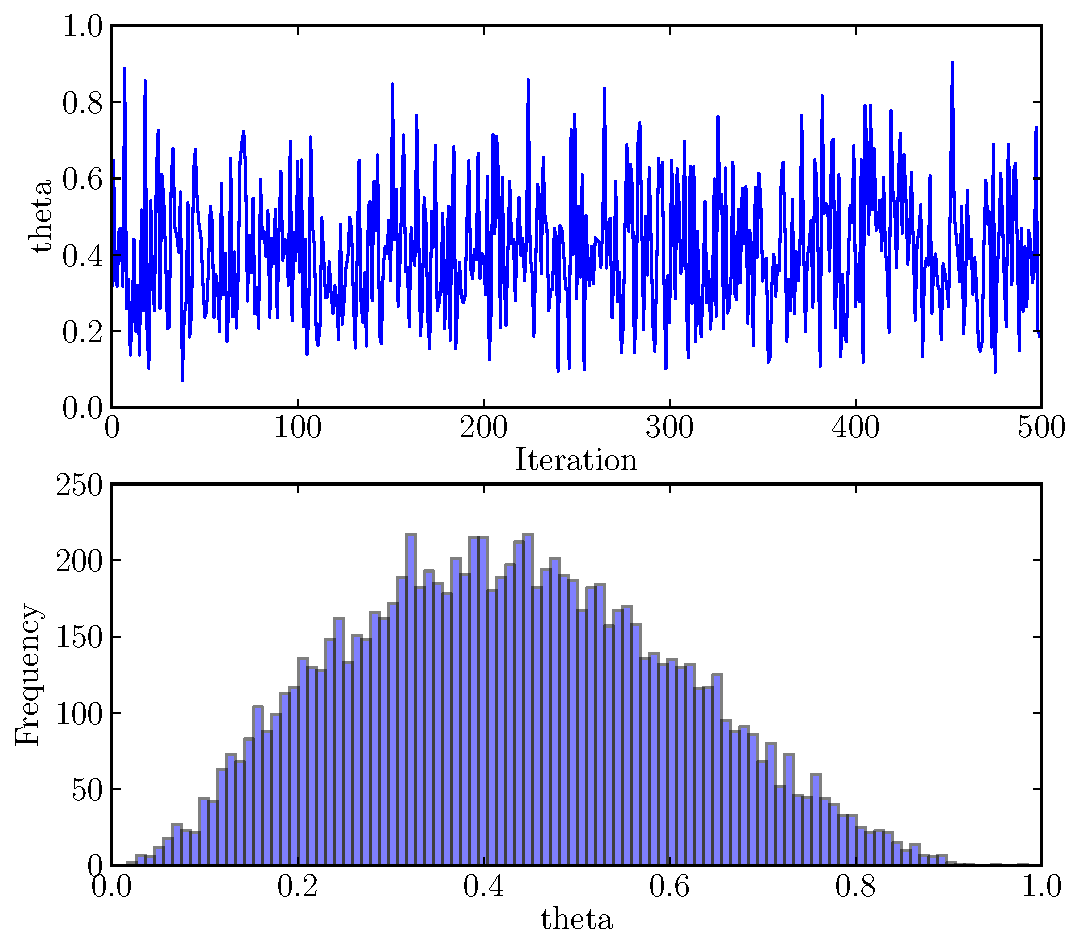
\includegraphics[scale=0.5]{Figures/jags_example.pdf}
\caption{\it The trace plot and histogram of the MCMC samples returned by
JAGS. The trace plot (top) is zoomed in on the first 500 samples, and shows the
{\tt theta} value moving around as the MCMC proceeds. The histogram of {\tt
theta} values, sampled from the posterior distribution, is given in the lower
panel. You can compare this with Figure~\ref{fig:bus_inference}.
\label{fig:results}}
\end{center}
\end{figure}

\section{Checklist for Using JAGS}
When running JAGS using the {\tt use\_jags.r} script provided, there are several
things you need to ensure. These are listed below.

\begin{itemize}
\item The data you want to analyse must be contained in an R
list called {\tt data}. Inside this list you should also include variables
such as the size of the data set (which I usually call {\tt N}),
or any other known constants that are
referred to in the model.
\item The JAGS model must be correctly written inside the R string called
{\tt model}. In the likelihood part of the JAGS model, you must ensure that
the names of the data variables match the names in your {\tt data} list. In
the example of this chapter, the number of successes is called {\tt x} in both
the data list and in the JAGS model.
\item The {\tt variable\_names} vector, which lists the parameters you are
interested in, can only list parameters that actually exist in the JAGS model!
\end{itemize}

\chapter{Regression}
Linear regression is a very important topic in statistics. It is also a nice
example to demonstrate how Bayesian statistics works and how it is different
from classical or frequentist statistics. Here we will study an example of a simple linear
regression problem, taken from STATS 201.

Data were collected from random sample of 30 drivers. The age of the driver and the 
maximum distance at which they could read a newly designed road sign were 
recorded. It is of interest to build a simple model that can be used to predict the 
maximum distance at which the sign is legible, using the age of the driver. The file 
{\tt road.txt} contains the data. Figure~\ref{fig:road} is a plot of the data:
\begin{figure}
\begin{center}
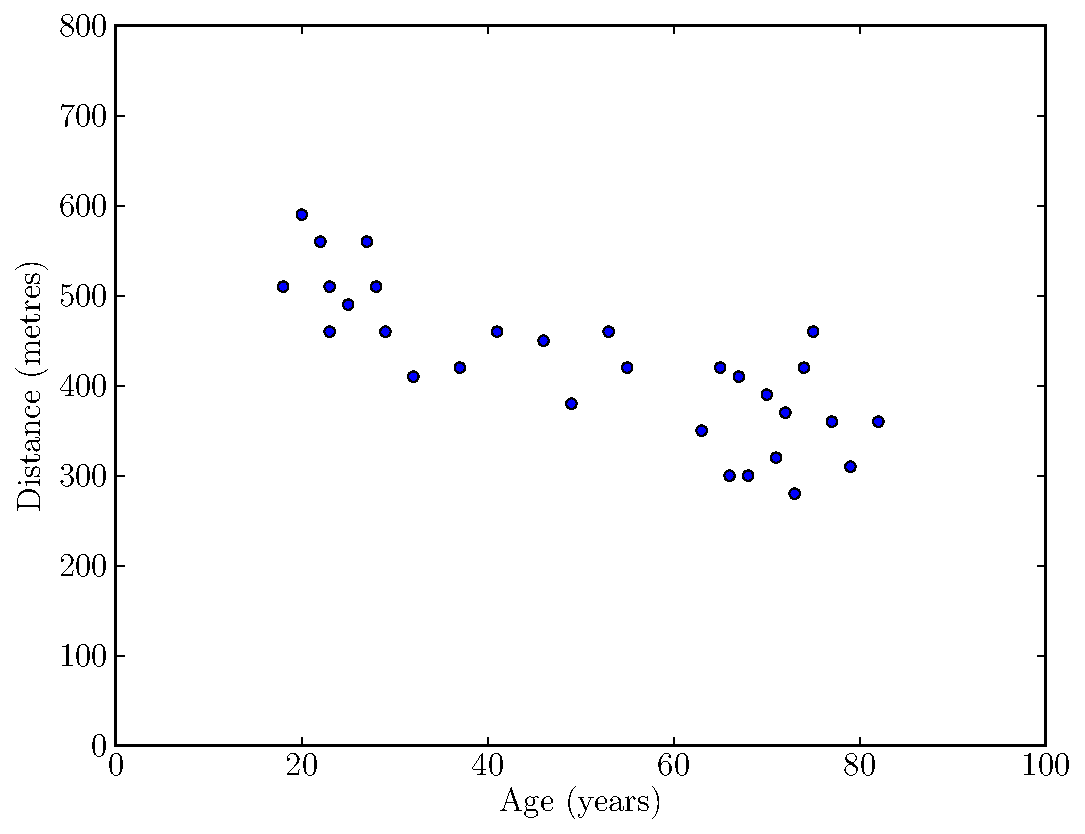
\includegraphics[scale=0.5]{Figures/road.pdf}
\caption{The distance at which a person can read a road sign, vs. the age of
the person. There are $N=30$ data points. You can clearly see that older people
have, on average, worse eyesight. But let's do a Bayesian analysis!\label{fig:ref}}
\end{center}
\end{figure}

\section{Simple Linear Regression}


\section{Analytical Solution With Known Variance}
The unknown parameters are $\beta_0$ and $\beta_1$, and the data are the
$y$ values. Bayes' rule (parameter estimation version) will give us the
posterior distribution:
\begin{eqnarray}
p(\theta|D) \propto p(\theta)p(D|\theta)
\end{eqnarray}

Let's assume a uniform prior:
\begin{eqnarray}
p(\beta_0, \beta_1) \propto 1.
\end{eqnarray}
Now, on to the likelihood. There are $N$ data points and so there are $N$
$y$-values in the dataset. We can call those $\{y_1, y_2, ..., y_N\}$. If we
knew the true values of $\beta_0$ and $\beta_1$, then we would predict the
$y$-values to be scattered around the straight line, with the probability
distribution for the amount of scatter given by a normal distribution with
standard deviation $\sigma$, and the amount of scatter is independent for
each data point. In statisticians' notation, this can be written as:
\begin{eqnarray}
y_i \sim \mathcal{N}(\beta_0 + \beta_1 x_i, \sigma^2).
\end{eqnarray}
The full equation for the likelihood is:
\begin{eqnarray}
p(y_i|\beta_0, \beta_1) &=& \prod_{i=1}^N \frac{1}{\sigma\sqrt{2\pi}}
\exp\left[-\frac{1}{2\sigma^2}\left(y_i - (\beta_0 + \beta_1 x_i)\right)^2\right].
\end{eqnarray}
Remember that when we combine the likelihood with the prior using Bayes' rule,
we can usually ignore any constant factors out the front that do not depend on
the parameters. This allows us to ignore the first part of the product, outside
the exponential.
\begin{eqnarray}
p(\beta_0, \beta_1 | y_1, y_2, ..., y_N) &\propto& p(\beta_0, \beta_1)
p(y_1, y_2, ..., y_N|\beta_0, \beta_1)\\
&\propto& \prod_{i=1}^N \exp\left[-\frac{1}{2\sigma^2}\left(y_i - (\beta_0 + \beta_1 x_i)\right)^2\right]\\
&\propto& \exp\left[-\frac{1}{2\sigma^2}\sum_{i=1}^N\left(y_i - (\beta_0 + \beta_1 x_i)\right)^2\right].
\end{eqnarray}






\section{Solution With JAGS}
The assumption is that the data are a list of measurements:
\begin{eqnarray}
D = \{y_1, y_2, ..., y_N\}.
\end{eqnarray}
Since we are talking about linear regression, we are going to assume that the
relationship between the $x$ and the $y$ variables is described by some
straight line, but there is noise around the straight line:
The linear regression model says:
\begin{eqnarray}
y_i &=& \beta_0 + \beta_1 x_i + \epsilon_i
\end{eqnarray}
If the $\epsilon_i$ values were all zero, then the points would all lie on
a perfectly straight line.

This gives us the likelihood.

The unknown parameters are the intercept of the straight line, the gradient of
the straight line, and the standard deviation of the noise.
\begin{eqnarray}
\boldsymbol{\theta} = \{\beta_0, \beta_1, \sigma\}.
\end{eqnarray}

In JAGS, the model looks like this:
\begin{verbatim}
model
{
    # Prior for all the parameters
    beta0 ~ dnorm(0., pow(1E3, -2))
    beta1 ~ dnorm(0., pow(1E3, -2))
    log_sigma ~ dunif(-10., 10.)
    sigma <- exp(log_sigma)

    # Likelihood
    for(i in 1:N)
    {
        y[i] ~ dnorm(beta0 + beta1*x[i], pow(sigma, -2))
    }
}
\end{verbatim}
The first part defines the priors for the parameters. For $\beta_0$ and $\beta_1$,
we have just chosen very broad priors that describe vague prior knowledge. Note
that the standard deviations of the priors are 1000, so we should be careful
to only apply this code to situtations where we don't expect the intercept or
slope to take on an extreme value.

For the standard deviation parameter $\sigma$ which describes how much we
expect the data points to be scattered around the straight line, we have assigned
a log-uniform prior. The limits of $-10$ and $10$ for {\tt log\_sigma} imply
limits of $4.5 \times 10^{-5}$ to 22,000 for {\tt sigma}, a generous range.
Again, if we thought the scatter
was going to be outside this range, we should change the prior to something
else.



\chapter{Simple Linear Regression With Outliers}


\chapter{ANOVA}
One-way ANOVA is a common procedure in statistics, and is related to the
simpler idea of a t-test. These classical tests were designed for particular
kinds of problems, and in this chapter we will study similar problems but
solve them from a Bayesian point of view.
We will also use these examples to discuss some issues about the choice
of prior distributions when there are more than a few parameters. When there
are only a few parameters it is usually safe to assign a vague, wide prior
to describe your initial uncertainty (unless, of course, you have more
information than that). In higher dimensions, problems can arise if you do
this. One way of getting around these problems is to use a
{\it hierarchical model}.

\section{A T-Test Example}
This example is based on one given in a 1976 article by physicist E. T. Jaynes,
called ``Confidence Intervals vs. Bayesian Intervals''. This is a very strongly
worded paper and might be an interesting read for
those who are interested in the battle between frequentist and Bayesian statistics
when the latter was making its comeback in the second half of the 20th century.
It's also where I got the crazy confidence interval example from.

Two manufacturers, $1$ and $2$, both make ``widgets'', and we are interested
in figuring out which manufacturer makes the best widgets (on average), as
measured by their lifetime. To determine this, we obtain 9 widgets from
manufacturer $1$ and 4 widgets from manufacturer $2$, and measure their
lifetimes, in days. The results are given below:
\begin{eqnarray}
x^1 &=& \{41.26, 35.81, 36.01, 43.59, 37.50, 52.70, 42.43, 32.52, 56.20\}\\
x^2 &=& \{54.97, 47.07, 57.12, 40.84\}
\end{eqnarray}
These measurements can be summarised by the means and standard deviations, which
are $42 \pm 7.48$ for group $1$ and $50 \pm 6.48$ for group $2$.
The question is: given this data, is there evidence that one of the manufacturers
is better than the other, and if so, by how much?
In classical statistics the standard procedure for this situation would be a
two sample $t$0-test. However, before we do anything I'd like you to consider
the numbers and use your intuition: what do {\it you} think about what the
evidence says?

An underlying assumption of a classical $t$-test is that the data are normally
distributed around the mean values for each group\footnote{Strictly speaking,
it's the probability distribution for the data given the parameters
that is normal, the data may or may not look normally distributed.}.
We may as well adopt this
assumption for our Bayesian model. If we call the group 1
data points $\{x^1_1, x^1_2, ..., x^1_{N_1}\}$ and the group 2 data points
$\{x^2_1, x^2_2, ..., x^2_{N_1}\}$, then the likelihood is:
\begin{eqnarray}
x^1_i &\sim& \mathcal{N}\left(\mu_1, \sigma^2\right)\nonumber\\
x^2_i &\sim& \mathcal{N}\left(\mu_2, \sigma^2\right)\label{eq:ttest_likelihood}
\end{eqnarray}
Where all the data points are independent given the parameters. Note the assumption that
the two groups have the same underlying (``population'') standard deviation $\sigma$. This is a popular
assumption in this kind of analysis but it is not necessarily well justified!
We will build our Bayesian models using this assumption, but it is not that
difficult to relax it if you want to. You could just include multiple
$\sigma$ parameters in the model,
just like how we will include the multiple $\mu$ parameters.

Instead of just one model for this situation, we will study three different
versions. Each model will have the same likelihood
as given above in Equation~\ref{eq:ttest_likelihood}, and the same prior
for $\sigma$. However, the models will all have different priors for $\mu_1$
and $\mu_2$.
We will be able to see that the choice of prior does
influence the results (of course), but in ways that make sense. Which of these
models is more appropriate in a practical situation would depend on the exact
situation. There is no ``one size fits all'' model.

\subsection{Likelihood}
To implement our model in JAGS, we can begin by specifying the likelihood
part like so:

\begin{framed}
\begin{verbatim}
    # Sampling distribution/likelihood
    for(i in 1:N1)
    {
        x1[i] ~ dnorm(mu1, 1/sigma^2)
    }
    for(i in 1:N2)
    {
        x2[i] ~ dnorm(mu2, 1/sigma^2)
    }
\end{verbatim}
\end{framed}
We have called our data arrays {\tt x1} and {\tt x2}, and we have also
assumed that the sample sizes {\tt N1} and {\tt N2} are defined, so our
{\tt data} list will need to be consistent with these choices. The parameters
we will be estimating are {\tt mu1}, {\tt mu2}, and {\tt sigma}, so we will
need to specify prior distributions for them. In the following sections, we'll
use the same prior for {\tt sigma}, so we may as well specify that now.
Let's use a log-uniform prior where $\sigma$ is between $e^{-10}$ and
$e^{10}$.

\begin{framed}
\begin{verbatim}
    # Prior for sigma
    log_sigma ~ dunif(-10, 10)
    sigma <- exp(log_sigma)
\end{verbatim}
\end{framed}

\subsection{Prior 1: Very Vague}
The last missing ingredients to finish the JAGS model are the priors for
{\tt mu1} and {\tt mu2}. For our first model, let's be really naive and assign
super-wide uniform priors.

\begin{framed}
\begin{verbatim}
    # Prior 1: Very Vague
    mu1 ~ dunif(-1000, 1000)
    mu2 ~ dunif(-1000, 1000)
\end{verbatim}
\end{framed}

At first glance, this might seem like a fairly reasonable thing to do. In many
problems, it doesn't make much difference if we just use vague priors and get
on with the calculation (as opposed to thinking really hard about the prior,
and what is actually known about the parameters).

However, this prior has a number of properties that suggest it might not be
quite right: firstly, what is the probability that $\mu_1 = \mu_2$?
In classical t-tests, the whole point is to test the hypothesis that
the two ``population means'' (parameters) are equal. However, our prior
actually implies that the probability they are equal is 0! Therefore, no matter
what data we get, the posterior probability of $\mu_1 = \mu_2$ will always be
zero.

\subsection{Prior 2: They might be equal!}
The problem with Prior 1 is that we may think $\mu_1$ might exactly equal
$\mu_2$, and Prior 1 doesn't allow for this. So here's another way we might
set up the prior. We'll start by defining the prior for $\mu_1$ as we did
before. Then, when we consider $\mu_2$, we need a way of giving it a
50\% probability of equalling $\mu_1$, and if not, then it should have
a uniform distribution between -1000 and 1000. Here is our solution. Read it
carefully and make sure you understand what this prior does.

\begin{framed}
\begin{verbatim}
    # First mean
    mu1 ~ dunif(-1000, 1000)

    # Prior on second mean, if it's different
    maybe ~ dunif(-1000, 1000)
    flag ~ dunif(0, 1)
    mu2 <- mu1 + (maybe - mu1)*step(flag - 0.5)
\end{verbatim}
\end{framed}

\subsection{Prior 3: Alright, they're not equal, but they might be {\it close}}
Prior 2 is also a little bit strange, if you think about it. If we're comparing
these two manufacturers of widgets, why would we think it is possible that the
two manufacturers are {\tt exactly} equal? Maybe we just think the parameters
$\mu_1$ and $\mu_2$ are likely to be {\it similar} in value.
In other words, we shouldn't worry so much about the
prior probablity of $\mu_1 = \mu_2$, but we should at least make sure there's
a moderate prior probability that $\mu_1 \approx \mu_2$.

One way we could do this is by applying a normal prior to both $\mu_1$ and
$\mu_2$ with some mean (let's call it the ``grand mean'')
and some standard deviation (let's call it the ``diversity'').
That way, $\mu_1$ and
$\mu_2$ would both be likely to be somewhere around the grand mean, and
they would likely be different by roughly the size of the diversity.
The challenge now seems to be the choice of appropriate values for the grand
mean and the diversity. Fortunately, we don't actually have to! What we can
do instead is apply priors for them instead.

This is our first example of a {\it hierarchical model}. In a hierarchical
model, instead of directly assigning priors to our parameters, we imagine that
we knew the values of some other parameters (called ``hyperparameters''), and
assign our prior for the parameters {\it given} the hyperparameters. Then we
assign a prior for they hyperparameters as well, to complete the model.

\begin{framed}
\begin{verbatim}
    # Hierarchical prior for the means
    # Hyperparameters
    grand_mean ~ dunif(-1000, 1000)
    log_diversity ~ dunif(-5, 5)
    diversity <- exp(log_diversity)

    # Prior for the parameters given the hyperparameters
    mu1 ~ dnorm(grand_mean, 1/diversity^2)
    mu2 ~ dnorm(grand_mean, 1/diversity^2)
\end{verbatim}
\end{framed}


Samples (obtained using JAGS) of the three priors are shown in
Figure~\ref{fig:ttest1}.
\begin{figure}[h]
\begin{center}
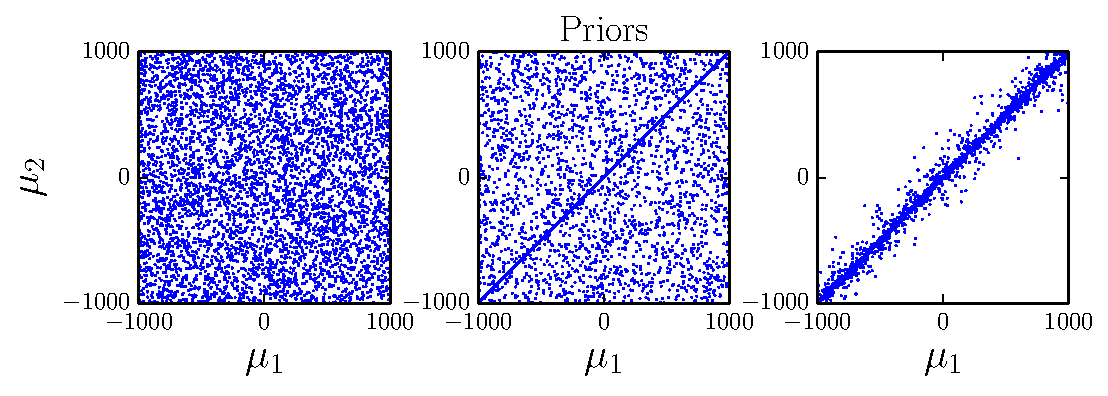
\includegraphics[scale=0.8]{Figures/ttest1.pdf}
\caption{\it The three different priors we are trying for our Bayesian
equivalent of a t-test. The first prior simply asserts a large amount of
prior ignorance about the value of the two parameters $\mu_1$ and $\mu_2$.
The second is similar but applies 50\% probability to the proposition
$\mu_1 = \mu_2$. The third prior does not allow the two parameters to be
exactly equal, but enhances the probability that they are quite similar
in value.\label{fig:ttest1}}
\end{center}
\end{figure}

The posteriors are shown in Figure~\ref{fig:ttest2}.
The inferences are different, as you would expect, and that's entirely down
to the choice of the prior. Any summaries we make will therefore depend on
which prior we want to use.
\begin{figure}[h]
\begin{center}
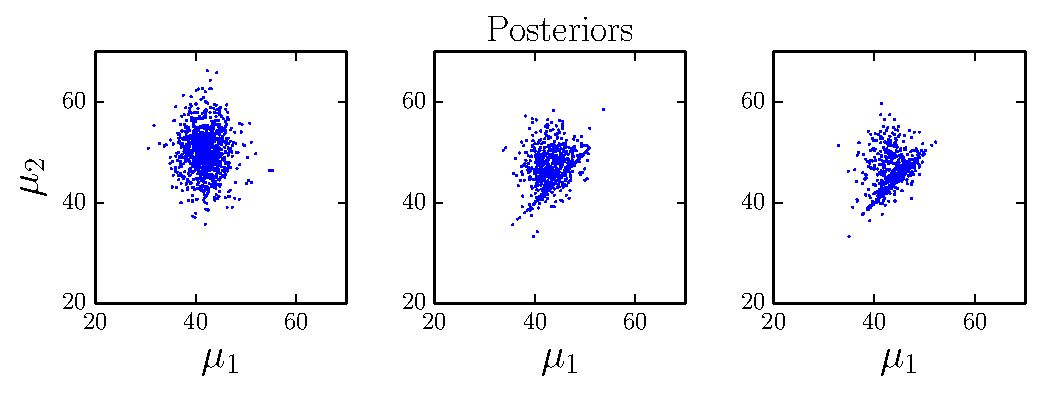
\includegraphics[scale=0.8]{Figures/ttest2.pdf}
\caption{\it The posterior distributions, given the widget data,
based on the three different priors for $\mu_1$ and $\mu_2$.\label{fig:ttest2}}
\end{center}
\end{figure}

The original question was whether manufacturer two was better, equal, or worse
than manufacturer one. We can answer that question by calculating the
posterior probabilities of $\mu_1 = \mu_2$, $\mu_1 < \mu_2$, and
$\mu_1 > \mu_2$. The results are shown in Table~\ref{tab:ttest_results}.

\begin{table}
\begin{center}
{\bf Prior Probabilities}:\\
\begin{tabular}{|l|c|c|c|}
\hline
Prior	&	$\mu_1 < \mu_2$	& $\mu_1 = \mu_2$	& $\mu_1 > \mu_2$\\
\hline
1 	&	0.5		&	0		&	0.5\\
2 	&	0.25		&	0.5		&	0.25\\
3 	&	0.5		&	0		&	0.5\\
\hline
\end{tabular}\\
{\bf Posterior Probabilities}:\\
\begin{tabular}{|l|c|c|c|}
\hline
Prior	&	$\mu_1 < \mu_2$	& $\mu_1 = \mu_2$	& $\mu_1 > \mu_2$\\
\hline
1 	&	0.5		&	0		&	0.5\\
2 	&	0.25		&	0.5		&	0.25\\
3 	&	0.5		&	0		&	0.5\\
\hline
\end{tabular}

\caption{\label{tab:ttest_results}}
\end{center}
\end{table}

Prior 1 ...
Prior 2 has bad mixing (and sensitivity to where we put the edge of the prior).
Prior 3 seems like it's what we might want in general.


\section{One Way Anova}
One-way ANOVA can be considered as a generalisation of a t-test to more than
two groups. The question is usually phrased as a test of the hypothesis that
the group means are the same, versus the alternative that there is some difference.
As we saw in the Bayesian ``t-test'', it is possible (using clever tricks) to
make a model that has some prior probability that the group means are equal.
However, this gets more tricky with multiple groups. Therefore we will build our
one-way ANOVA model in a similar way to the ``hierarchical model'' version of the
t-test model. There will be one other major difference, but it is a difference
in the way the model is coded, not a conceptual difference. In the t-test
section we used different 

The masses of starlings were measured at four locations.

\begin{figure}[ht!]
\begin{center}
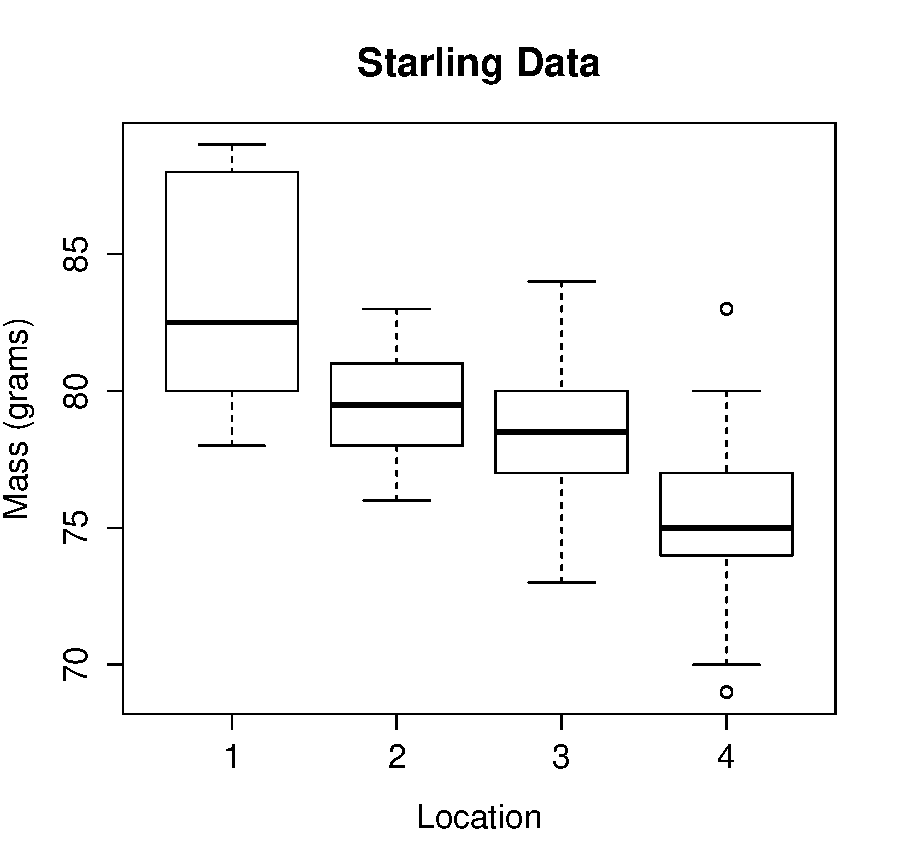
\includegraphics[scale=0.6]{Figures/starling.pdf}
\end{center}
\end{figure}


\subsection{Hierarchical Model}
The main advantage of this model is that it generalises to more than two groups
in a very straightforward way. The difference is the prior. Whereas the first
model had independent priors for the means of the groups, this version is our
first example of a {\it hierarchical model}.
\begin{framed}
\begin{verbatim}
model
{
    # Log-uniform prior for the scatter
    log_sigma ~ dunif(-10, 10)
    sigma <- exp(log_sigma)

    # Hierarchical prior for the means
    # Hyperparameters
    grand_mean ~ dnorm(0, 1/1000^2)
    log_diversity ~ dunif(-10, 10)
    diversity <- exp(log_diversity)

    # Parameters
    mu1 ~ dnorm(grand_mean, 1/diversity^2)
    mu2 ~ dnorm(grand_mean, 1/diversity^2)

    # Sampling distribution/likelihood
    for(i in 1:N)
    {
        x[i] ~ dnorm(mu[group[i]], 1/sigma^2)
    }
}

\end{verbatim}
\end{framed}




\appendix
\chapter{R Background}

This chapter describes the R programming techniques that we will need.


\appendix
\chapter{Probability}
This course will use probability theory extensively.

The product rule:
\begin{eqnarray}
P(A, B) &=& P(A)P(B|A) \\
&=& P(B)P(A|B)
\end{eqnarray}

The sum rule:
\begin{eqnarray}
P(B) &=& P(A)P(B|A) + P(~A)P(B|~A) \\
&=& P(B)P(A|B)
\end{eqnarray}



\appendix
\chapter{Rosetta Stone}
Bayesian statistics has a lot of terminology floating around, and sometimes
different communities use different terms for the same concept. This appendix
lists various terms that are are basically synonymous (they mean the same thing).
I may even throw in the different terms from time to time, intentionally or
unintentionally!

{\bf Event, Hypothesis, Proposition, Statement}\\
These are all basically the same thing.
A statement is something that can be either true or false, such as ``my age is
greater than 35''. These are the things that go in our
probability statements: If we write $P(A|B)$, $A$ and $B$ are both propositions,
that is, statements that may be true or false. Event is the preferred term in
classical statistics.

{\bf Sampling Distribution, Probability Model for the Data, 
Generative Model, Likelihood Function, Likelihood}\\
This is the thing that we
write as $p(D|\theta)$. Sometimes it is called the sampling distribution or
a generative model because
you can sometimes think of the data as having been ``drawn from''
$p(D|\theta)$ but using the true value of $\theta$, which you don't actually
know. There is a subtlety here, and that is that the word likelihood can be
used to mean either $p(D|\theta)$ before $D$ is known (in which case it is the
thing you would use to predict possible data) or after $D$ is known. In the latter
case $p(D|\theta)$ is only a function of $\theta$ because $D$ is fixed at the
observed value. The term likelihood function is often used at this point.

{\bf Probability Distribution} is used to describe either the probability density
function (in the continuous case) or a probability mass function (in the discrete
case). The latter gives the probability of each particular value, whereas the
former only gives a probability if you integrate it within some region.

{\bf Marginal Likelihood, Evidence, Prior Predictive Probability, Normalising
Constant}\\ This is the $p(D)$ or $P(D)$ term in the denominator of Bayes' rule,
and it is also the total of the {\tt prior} $\times$ {\tt likelihood} column
of a Bayes' Box. This is the probability of getting the data that you actually got,
before you observed it: hence the terminology ``prior predictive probability''.
It is also the thing you use to normalise the posterior distribution (make it sum
or integrate to 1), hence the term normalising constant. Marginal likelihood makes
sense because it is a probability of data (like the regular likelihood) but
``marginalised'' (i.e. not caring about) the value of the parameter(s). It is
also called ``evidence'' because it can be used to compare different models, or
to ``patch together'' two Bayes' Boxes after the fact (see the hypothesis testing
chapter).



\end{document}

